% =====================================================================
%  49274 Space Robotics - Team Project: Exploring a Martian Cave
%  Single-file report. Compile with: make   (pdflatex x2)
%
%  DRAFT written by Karan Sharma (report lead). Everything marked
%  "TODO" or "STUDENT ACTION REQUIRED" must be completed or checked by
%  the named person before submission. Search for TODO.
%
%  The only other input is the auto-generated table of Gazebo results,
%  generated/sampling_table.tex, made by scripts/sampling_summary.py.
% =====================================================================
\documentclass[11pt,a4paper]{article}

\newcommand{\reporttitle}{Team Project: Exploring a Martian Cave}
\newcommand{\reportsubtitle}{Autonomous perception, planning and science for a Mars rover}
\newcommand{\studentname}{Than, Li, Sharma}
\newcommand{\subjectname}{49274 Space Robotics}
\newcommand{\institution}{University of Technology Sydney}
\newcommand{\reportdate}{October 2026}

% =====================================================================
%  Shared preamble - packages, colours, heading style, code listings.
%  Kept close to the Assessment task 1 report look.
% =====================================================================

\usepackage[T1]{fontenc}
\usepackage[utf8]{inputenc}
\usepackage[margin=1in]{geometry}
\usepackage{amsmath,amssymb}
\usepackage{graphicx}
\usepackage{xcolor}
\usepackage{booktabs}
\usepackage{array}
\usepackage{enumitem}
\usepackage{titlesec}
\usepackage{fancyhdr}
\usepackage[labelfont={bf,color=sectionblue}]{caption}
\usepackage{listings}
\usepackage[most]{tcolorbox}
\usepackage[colorlinks=true,linkcolor=sectionblue,urlcolor=sectionblue,citecolor=sectionblue]{hyperref}

% ---------------------------- Colours --------------------------------
\definecolor{sectionblue}{HTML}{1F6FB2}
\definecolor{codebg}{HTML}{F5F5F5}
\definecolor{codekw}{HTML}{1F6FB2}
\definecolor{codecomment}{HTML}{7A7A7A}
\definecolor{codestring}{HTML}{A31515}
\definecolor{notegreen}{HTML}{157F7A}

% ------------------------- Heading style -----------------------------
\titleformat{\section}
  {\color{sectionblue}\bfseries\large}{\thesection}{0.6em}{}
\titleformat{\subsection}
  {\bfseries\normalsize}{\thesubsection}{0.6em}{}

% "N marks" badge next to a task heading
\newcommand{\taskmarks}[1]{%
  \hspace{0.5em}\raisebox{0.12ex}{\colorbox{sectionblue}{\color{white}\scriptsize\,#1 marks\,}}}

% ------------------------- Page headers ------------------------------
\pagestyle{fancy}
\fancyhf{}
\renewcommand{\headrulewidth}{0.4pt}
\lhead{\color{sectionblue}\small \reporttitle}
\rhead{\color{gray}\small \studentname}
\cfoot{\thepage}

% ------------------------ Code listings -----------------------------
\lstdefinestyle{py}{
  language=Python,
  backgroundcolor=\color{codebg},
  basicstyle=\ttfamily\footnotesize,
  keywordstyle=\color{codekw}\bfseries,
  commentstyle=\color{codecomment}\itshape,
  stringstyle=\color{codestring},
  numbers=left,
  numberstyle=\tiny\color{codecomment},
  numbersep=8pt,
  frame=single,
  rulecolor=\color{gray!40},
  breaklines=true,
  showstringspaces=false,
  captionpos=b,
  xleftmargin=2.2em,
  framexleftmargin=2em,
  aboveskip=1em,
  belowskip=1em,
}
\lstset{style=py}

% ---------------------- Note / callout box --------------------------
\newtcolorbox{notebox}[1][Note]{
  colback=notegreen!6, colframe=notegreen, coltitle=white,
  fonttitle=\bfseries, title=#1, boxrule=0.6pt, arc=1pt,
  left=6pt, right=6pt, top=4pt, bottom=4pt}

% ---------------------- Placeholder figure --------------------------
% Use where a real RViz screenshot is still needed. Prints a visible
% grey box so nothing silently ships empty. Replace with \includegraphics.
\newcommand{\figplaceholder}[1]{%
  \begingroup\centering
  \fcolorbox{gray!50}{gray!12}{\parbox[c][3.2cm][c]{0.75\linewidth}{\centering
  \color{gray!80}\ttfamily\footnotesize [TODO screenshot] #1}}\par
  \endgroup}

\graphicspath{{../figures/}}

\newcommand{\todo}[1]{\textcolor{red}{\textbf{[TODO: #1]}}}

\begin{document}

% ------------------------------- Title -------------------------------
\begin{center}
    {\color{sectionblue}\bfseries\large 49274 --- Space Robotics}\\[0.5em]
    {\color{sectionblue}\bfseries\huge \reporttitle}\\[0.3em]
    {\large \reportsubtitle}\\[0.6em]
    {\small Andrew Than, Christina Li, Karan Sharma \quad\textbullet\quad \institution \quad\textbullet\quad \reportdate}
\end{center}
\vspace{0.5em}

% =====================================================================
\section{Group Member Details}

\begin{center}
\begin{tabular}{@{}p{3cm}p{4.6cm}p{6.6cm}@{}}
\toprule
\textbf{Name} & \textbf{Student number} & \textbf{Main responsibility} \\
\midrule
Andrew Than  & 13223096 & Perception (tasks P1--P3) \\
Christina Li & 25730019 & Planning (tasks L1--L3) \\
Karan Sharma & 26276485 & Advanced tasks A2 and A6; report lead; repository \\
\bottomrule
\end{tabular}
\end{center}

\noindent Task labels: P1--P3 are Perception 1--3, L1--L3 are Planning 1--3, and A2 and A6 are
Advanced 2 (cave geometry analysis) and Advanced 6 (adaptive scientific sampling).

% =====================================================================
\section{Generative AI Disclosure}

\textbf{Karan Sharma.} Claude Code (Anthropic) was used throughout: it wrote first versions of the cave geometry and adaptive sampling code,
the artefact detectors with the trained box check and the live artefact placement, the inspection timeout and close-range confirmation fixes in the explorer node,
and the test scripts, and it drafted the project plan and this report. It was not used to choose the NASA data set, run the demonstration or record the video, and each
component was run in the simulator and scored against the world-file truth before it was accepted.

\textbf{Andrew Than.} Microsoft Copilot was used to correct syntax and logic errors, debug the Perception~1 code, integrate a Google Teachable Machine model into ROS~2,
recommend OpenCV libraries for Perception~2 and add separate markers for each artefact type in Perception~3. \todo{Andrew: one sentence on what Copilot was not used for and what you can explain unaided.}

\textbf{Christina Li.} ChatGPT (OpenAI) was used to explain ROS~2 and Nav2 concepts, to develop and debug the planning code, to diagnose navigation problems and to check the wording
of the Planning sections, but not to produce experimental results or demonstration footage. Exploration, inspection and behaviour switching were tested in the simulator (Ubuntu, ROS~2, Gazebo, RViz),
and the report was checked against the observed results.

% =====================================================================
\section{Statement of Individual Contributions}

\begin{notebox}[STUDENT ACTION REQUIRED --- every member]
The ``Completed?'' entries below are Karan's reading of the repository and must be corrected by the
member who owns each row. Anyone who disagrees with the statement may write to the Subject
Coordinator privately.
\end{notebox}

\begin{center}
\small
\begin{tabular}{@{}p{3.1cm}p{2.7cm}p{2.5cm}p{6.2cm}@{}}
\toprule
\textbf{Task} & \textbf{Completed?} & \textbf{Member} & \textbf{Contribution} \\
\midrule
Perception 1 (dataset) & Yes & Andrew Than & Image-saving code in the ROS node; 100-image dataset. \\[3pt]
Perception 2 (detection) & Alien and crystal & Andrew Than &
  First colour detector (green objects). \\
 & Yes, additional detectors & Karan Sharma &
  Alien, crystal, mushroom, sphere and ice detectors, trained box check, live detection and artefact markers in the node, simulator capture and scoring scripts (Section~\ref{sec:perception}). \\[3pt]
Perception 3 (localisation) & Partly & Andrew Than & Distance from the depth camera, marker placement and a 2\,m merge rule (first version, on the \texttt{perception} branch); the final module builds on it. \\[3pt]
Planning 1 (exploration) & Yes & Christina Li & Frontier exploration. \\[3pt]
Planning 2 (inspection) & Yes & Christina Li & Stand-off approach goal and inspection. \\[3pt]
Planning 3 (switching) & Yes & Christina Li & Explore--inspect state machine with timeout, retry and visited record. \\[3pt]
Advanced 2 (geometry) & Yes & Karan Sharma & Design, code, simulator tests, evidence. \\[3pt]
Advanced 6 (sampling) & Yes & Karan Sharma & Design, code, simulator tests, comparison. \\[3pt]
Report writing & In progress & Karan Sharma (lead), all & Karan edits and unifies; each member writes their own task section. \\[3pt]
Recorded videos & Planning: yes & Christina Li & Planning 1--3 simulator demonstrations using Gazebo and RViz. Andrew: not recorded. \todo{Karan: add the Advanced videos.} \\
\bottomrule
\end{tabular}
\end{center}

% =====================================================================
\section{Project Overview}

The task is to program a simulated Mars rover to explore an unknown lava-tube-like cave without
human input: build a map, find artefacts of scientific interest, and understand the environment. The
cave is a Gazebo world of walls and 14 artefacts of five types (green alien, green crystals, white
sphere, blue mushrooms, ice formations) plus stop signs. The rover carries a laser scanner, an RGB
camera and a depth camera; \texttt{slam\_toolbox} builds the map and Nav2 plans and drives to goals.

The team split the work into three parts. \textbf{Perception} detects and localises
artefacts from the camera. \textbf{Planning} chooses where to go, switches between
exploring and inspecting, and keeps a record of visited artefacts. \textbf{Advanced} analyses
the cave geometry as it is explored and samples a spatial science field adaptively.

\paragraph{Status at the time of writing (17 October 2026).}
\begin{itemize}[nosep]
  \item \textbf{Advanced 2 and Advanced 6} are complete and on \texttt{main}. Both were run in Gazebo with real navigation and a
        real SLAM map. The cave geometry analysis found the widest open area and the narrow passages. The adaptive sampler took 30
        readings of a real NASA water map in each of 12 runs.
  \item \textbf{Perception.} An image saver and a colour detector for green objects are on \texttt{main}. The red-octagon stop-sign
        classifier is also on \texttt{main} and is called by the exploration node. Detectors for the alien,
        crystal, mushroom, sphere and ice are scored offline on saved images and are not called by the node
        (Section~\ref{sec:perception}). Locating artefacts on the map (Perception~3) is not on the repository.
  \item \textbf{Planning.} Exploration, inspection and behaviour switching are on \texttt{main} through the integrated
        exploration node described in Section~\ref{sec:planning}.
  \item \textbf{Integration.} The autonomy launch runs exploration, inspection and the stop-sign detector together. Perception~1--3
        and the other artefact detectors are not part of that run. The Advanced tasks run as separate launches.
\end{itemize}
\todo{All: update this list to the final state before submission. Do not overstate what was achieved.}

\paragraph{Software layout.}
All code is in one ROS~2 package, \texttt{cave\_explorer}, in a shared Git repository, with one
folder per part (\texttt{perception/}, \texttt{planning/}, \texttt{advanced/}). Tests that need no
simulator and the scripts used for every figure are in \texttt{scripts/}. The Advanced tasks run as
their own nodes, so they do not edit the shared node that the other parts use.

\paragraph{Building on earlier assignments.}
Several methods in this project were first met in the earlier assignments of the subject (Assignment 1, particle filter localisation,
and Assignment 2, path planning, both 49274 Space Robotics, Spring 2026). Table~\ref{tab:prior} shows where each one is used and how it
differs from the earlier version. Methods that were not needed are listed as well.

\begin{table}[h]
\centering
\caption{Ideas from the earlier assignments and their use in this project.}
\label{tab:prior}
\small
\begin{tabular}{@{}p{3.3cm}p{4.3cm}p{4.9cm}@{}}
\toprule
\textbf{From} & \textbf{Used here for} & \textbf{Difference from the earlier version} \\
\midrule
Assignment 2, Dijkstra's algorithm (core concept, extended to A* in Task 3) & Path length from the rover to each frontier (Planning 1) and to each sampling candidate (Advanced 6). & Run once from the rover over all cells, with no goal node and no energy cost. A* heuristic is not used, since there is no single goal. \\[4pt]
Assignment 2, distance transform (Task 9) & Distance from each free cell to the nearest wall: the basis of the widest-area and passage analysis (Advanced 2). & Exact Euclidean transform from SciPy, not the two-pass approximation. \\[4pt]
Assignment 2, medial axis as an optional extension (Task 10) & The centre-line of the cave, found where the distance stops changing at one metre per metre (Advanced 2). & A gradient threshold locates the centre-line. A Hessian test classifies saddle points. A cut test decides which candidates are narrow passages. \\[4pt]
Assignment 2, probabilistic roadmap (Tasks 7 and 10) & Not used. The SLAM occupancy grid is already dense, so candidate points are taken from the grid. & Would be needed for a larger map with no grid, or for many-goal planning. \\[4pt]
Assignment 1, particle filter (weighted particles as a belief, estimate from the weights) & Advanced 6 keeps a belief over the water field. The belief is a Gaussian Process (mean and variance), and its uncertainty chooses the next sample. & No particles and no motion model. The field is a function over space, learned from the rover's measurements. \\
\bottomrule
\end{tabular}
\end{table}

% =====================================================================
\section{Perception}
\label{sec:perception}

\begin{notebox}[STUDENT ACTION REQUIRED --- Andrew]
Perception 1, 2 and 3 now have text, written from Andrew's notes and the code. Andrew checks each of the three subsections
against what he did and corrects anything that is wrong, and adds RViz screenshots from his own runs if he has them.
\end{notebox}

\subsection{Perception 1 --- Image dataset}
\label{sec:p1}
\paragraph{Method.} The aim of Perception~1 was to collect a dataset of artefact images from the rover's onboard RGB camera.
Images are saved automatically while the rover explores, so the dataset grows without manual effort. The camera feed is read
from the ROS~2 \texttt{camera/image} topic, and each frame received by the image callback is converted to OpenCV format with
\texttt{CvBridge}. A dataset directory is created at start-up, and a frame is saved every 3\,s. The interval avoids
near-identical consecutive frames and limits storage use. Each file is named after its timestamp, so the images are unique and
in time order (Listing~\ref{lst:p1}).

\begin{lstlisting}[caption={Saving one camera frame every 3\,s (\texttt{perception/dataset\_collector.py}).},label={lst:p1},float=htb]
# Set-up: create the dataset folder and the save interval
self.dataset_directory_ = os.path.expanduser("~/artifact_dataset")
os.makedirs(self.dataset_directory_, exist_ok=True)
self.last_image_save_time_ = 0.0
self.save_interval_ = 3.0  # seconds between saved images

# In image_callback: save one frame every save_interval_ seconds
if current_time - self.last_image_save_time_ > self.save_interval_:
    filename = f"image_{int(current_time)}.png"
    filepath = os.path.join(self.dataset_directory_, filename)
    cv2.imwrite(filepath, image)
    self.last_image_save_time_ = current_time
\end{lstlisting}

\paragraph{Results.} The collector ran throughout exploration and captured artefacts from a range of distances, orientations
and viewpoints without human input. Figure~\ref{fig:p1} shows one example of each artefact type and a negative example with no
artefact. Because the images were collected during autonomous exploration, the number of images of each type depends on the
rover's path: artefacts that stayed in view for longer contributed more images, so the dataset is imbalanced
(Table~\ref{tab:p1}). Spheres and stop signs were seen most often and the alien least. Some images show more than one artefact, so the 100 images contain 172 artefact views in total. All images were collected
with no manual intervention.

\begin{figure}[h]
  \centering
  \newcommand{\pimg}[2]{\begin{minipage}[b]{0.135\linewidth}\centering
    \includegraphics[width=\linewidth,height=2.2cm,keepaspectratio]{perception1/#1}\\[-1pt]{\scriptsize #2}\end{minipage}}
  \pimg{alien.png}{Alien}\hfill\pimg{crystal.png}{Crystal}\hfill\pimg{ice.png}{Ice cap}\hfill
  \pimg{sphere.png}{Sphere}\hfill\pimg{mushroom.png}{Mushroom}\hfill\pimg{stop_sign.png}{Stop sign}\hfill
  \pimg{nothing.png}{Nothing}
  \caption{Example dataset images for each artefact type and a negative example, from the rover camera during exploration.}
  \label{fig:p1}
\end{figure}

\begin{table}[h]
\centering
\caption{Artefact images collected in 5 minutes of exploration. One image can show several artefacts, so the counts add up to 172 for 100 images.}
\label{tab:p1}
\small
\begin{tabular}{@{}lccccccc|r@{}}
\toprule
 & \textbf{Alien} & \textbf{Crystal} & \textbf{Ice cap} & \textbf{Sphere} & \textbf{Mushroom} & \textbf{Stop sign} & \textbf{Nothing} & \textbf{Images saved} \\
\midrule
\textbf{Images showing it} & 4 & 17 & 23 & 41 & 13 & 73 & 1 & \textbf{100} \\
\bottomrule
\end{tabular}
\end{table}

\paragraph{Limitations and improvements.} All images are saved to a single directory, and the artefact class of each image is
not recorded, so the images had to be inspected and sorted by hand before use. The class balance also depends on the
navigation path, which leaves some classes with far fewer images than others. Images could be labelled automatically: once the
perception system detects an artefact, the frame could be saved into a folder for that class, together with metadata such as
the artefact distance, rover pose and timestamp. A more structured exploration strategy, or a cap on images per class, would
give a more balanced dataset.

\subsection{Perception 2 --- Artefact detection in the running node}
\label{sec:p2}
\paragraph{Method and libraries.} Every camera frame passes through three detectors, and each detection is drawn as a labelled
bounding box on the \texttt{detections\_image} topic, which RViz shows in the Detections panel (Figure~\ref{fig:p2live}). Stop signs are found
by a rule-based red-octagon detector. The alien, crystals, mushroom and sphere are found by colour ranges in HSV space, and a
trained random forest then accepts or rejects each box. Ice is found by a per-pixel random forest on colour, texture and depth.
The design and scoring of each detector are described in Section~\ref{sec:p2detail}. The libraries are OpenCV and NumPy for the image
processing, \texttt{cv\_bridge} to convert ROS images, and scikit-learn to train the two forests.

\paragraph{The box check.} Colour alone cannot separate the alien and crystals from the green trees printed on the stop-sign
pictures that hang on some walls: a single green range found only 30\,\% of aliens, and the per-type ranges still box the trees. A
random forest (\texttt{perception/box\_classifier.py}) therefore looks at each candidate box and decides from about 25 numbers: the colour
of the matching pixels, texture (leaves are busy, artefact surfaces are smooth), the box size scaled by its distance, and depth (an artefact
stands in front of the wall, a picture lies flat on it). It was trained on 387 boxes from the labelled captures: those around the artefacts,
those in front of the stop-sign pictures and those in front of the timeline posters. On cave areas held out of training it keeps 95\,\% of
the real boxes and removes 94\,\% of the false ones, including all 127 false alien boxes (most of them trees on the pictures).

\paragraph{Integration with ROS.} Two problems came from running the detectors inside the ROS~2 node. First, a newer NumPy in the user's
Python packages breaks \texttt{cv\_bridge}, so the node runs with the system packages only. The forests are therefore exported to plain
arrays (an \texttt{.npz} file) and evaluated with NumPy, which needs no scikit-learn and takes about 0.5\,ms per box. Second, the ice forest
classifies every pixel and takes about 0.4\,s per frame, so it runs in a background thread every 2\,s and is switched off by default (the
parameter \texttt{detect\_ice}). The remaining detectors cost about 3\,ms per frame and do not slow the navigation. The ROS images arrive in
RGB order and are converted to BGR before detection, and the rover's own arm, which fills the lower-left of the image, is masked out.

\begin{table}[h]
\centering
\caption{Detection rates of the running pipeline on the labelled simulator captures. An artefact counts as found when a box covers it among
the images where it is in view, 1--9\,m away with a clear line of sight. The box check is scored on cave areas it was not trained on.}
\label{tab:p2rate}
\small
\begin{tabular}{@{}lcccc@{}}
\toprule
\textbf{Type} & \textbf{1--3 m} & \textbf{3--5 m} & \textbf{5--9 m} & \textbf{All} \\
\midrule
Alien     & 19/19 & 8/8   & 10/10 & 37/37 (100\,\%) \\
Crystals  & 17/20 & 9/9   & 5/5   & 31/34 (91\,\%) \\
Mushroom  & 25/25 & 11/11 & 11/11 & 47/47 (100\,\%) \\
Sphere    & 18/23 & 6/9   & 6/10  & 30/42 (71\,\%) \\
Stop sign & ---   & 22/23 & 6/9   & 28/32 (88\,\%) \\
Ice (optional) & \multicolumn{3}{c}{18 of 33 images that show it} & 55\,\% \\
\bottomrule
\end{tabular}
\end{table}

\paragraph{Results.} Table~\ref{tab:p2rate} gives the detection rates. False boxes appear in 11 of 218 images with no artefact in view
(5\,\%) and, for stop signs, in 2 of 233 images without a sign (1\,\%); the poster walls produce none. The sphere is the weakest
type: it is a pale blue-white ball against walls of a similar colour, and it is found in only 60\,\% of views from 5--9\,m. Ice is found in
about half of the images that show it, and in one live run a wall was boxed as ice, so it is not enabled by default.
All thresholds were chosen on these same captures and the box check was tested only on held-out places, so the rates are likely higher than a new
scene would give.

\begin{figure}[h]
  \centering
  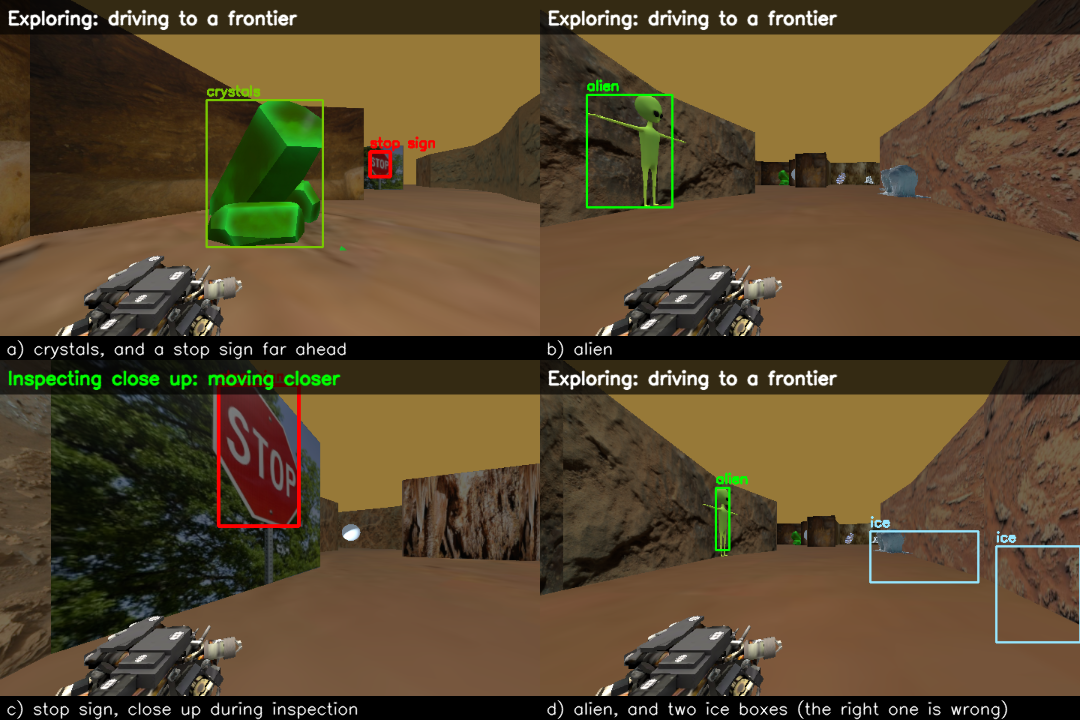
\includegraphics[width=0.8\linewidth]{perception2_live_detections.png}
  \caption{The Detections panel during a simulator run. The task the rover is carrying out is written along the top. (a)~Crystals, and a stop
  sign far ahead. (b)~An alien. (c)~A stop sign during close-range inspection. (d)~An alien and two ice boxes; the right-hand ice box is a
  false detection on the wall.}
  \label{fig:p2live}
\end{figure}

\subsection{Perception 2 --- Detector design and scoring}
\label{sec:p2detail}

\paragraph{Why a test set was needed.}
To measure the detectors, the rover was teleported to many viewpoints around each artefact in the
simulator and records the camera and depth images (405 images). The world file gives the true
position of each artefact, so each image is labelled with which artefact types are actually in view
(1--9\,m away, with a clear line of sight). The labels are used only to find colours and to score
detectors; the detectors see only the image.

\paragraph{Colour detectors.}
Each type has a distinct colour. The alien is pale lime (saturation 160--180), the crystals deep
emerald (saturation 204--255), the mushroom caps saturated blue (hue 110--112) and the sphere
pale blue-white (hue 105, saturation about 49). A mask per type, cleaned with morphological opening and
closing, gives boxes. The rover's own body, which fills the bottom-left of every frame, is blanked out.
The alien and crystals are told apart by saturation alone. On the 405 captured images the per-type ranges find 100\,\% of the aliens (33/33) and 95\,\% of the crystals (39/41), where one green range for all green objects finds only 30\,\% (10/33) and 66\,\% (27/41).



\paragraph{Ice needed a different method.}
Ice is hard for three reasons found by measurement. Each formation is about $5\times5\times1.5$\,m,
and the point used by the world file lies up to 3\,m from its centre, so a point label was wrong.
Its pixels are about half blue-grey and half brown-beige, the same colour as the cave walls and floor,
so no colour range works: a learned colour rule finds 15--21\% of ice and puts a false box in 62--82\% of
images. The detector in \texttt{ice\_detector.py} therefore classifies pixels with a random forest using
colour, local texture and two depth features (height above the floor and surface bumpiness). True ice
pixels for training and scoring come from projecting the ice mesh into each image and keeping the points
whose range agrees with the depth image. Trained on half the images and scored on the other half, it finds
ice in 18 of 33 images that show it (55\%), with a false ice box in 5\% of images, at 62\,ms per frame.
The detector is usable, but its reliability is limited.


\paragraph{Stop signs: a red-octagon classifier.}
The template's stop-sign detector is a Haar cascade (a trained pattern matcher). Some walls of the cave carry
the Mars timeline poster, which has framed year labels, and the cascade fires on them. In simulator runs of the
exploration code with the cascade, this produced 22 to 27 ``artefacts'' although the cave holds only five real stop signs.
A rule-based classifier is therefore used (\texttt{stop\_sign\_detector.py}, no trained weights) that checks the defining features of a stop sign:
strongly red pixels, a solid blob that is roughly square and fills about 83\,\% of its bounding box, an outline with about eight corners,
and pale lettering inside (red has high colour saturation, the letters low). The numeric limits were measured from
the simulator's sign photo (red value about 87, saturation about 212).

To score it, the rover was teleported around every real sign. For each of the five signs there are 5 photos on an arc in front of the sign,
28$^\circ$ apart (from $-56^\circ$ to $+56^\circ$, a $140^\circ$ cone) at about 4\,m; one of the 25 is impossible
because the rover cannot get 4\,m from that wall at $-56^\circ$, so there are 24. Another 193 photos look at every other wall (including the poster walls),
24 look at artefacts and 40 are random views, and a second set of 40 photos shows the seven poster walls from both sides (a deliberately difficult
test set). The world file says where every sign is, so each photo is labelled automatically; the detectors only see the image.
A box counts as a false alarm only if no real sign lies in that direction at any distance (13 of 15 boxes first counted as false were real, distant signs).



The cascade finds 26 of 32 signs within 9\,m and the red-octagon classifier 28. On the 233 photos with no sign in view the cascade gives 1 false box and the classifier 2, and on the 48 poster-wall photos the cascade gives 5 and the classifier none. The classifier removes the poster false alarms and finds slightly more signs. Its two false boxes (one on a rock wall, one in a random view)
are small and narrow; they are not explained. The photos used to choose the limits are the photos used to score it, so the numbers are optimistic.

\paragraph{Limits.}
Colour ranges were measured in this one world and tuned on the same 405 images, so the results above
are optimistic for a new scene or a fresh set of viewpoints. The detectors return a box and image
column; turning that into a map position (Perception~3) needs the depth image and the robot pose.
The stop-sign, colour and box-check detectors run in the rover's image callback (Section~\ref{sec:p2}); the ice detector runs there only when it is switched on.
The image passed to them must be in BGR order; ROS images arrive as RGB.

\subsection{Perception 3 --- Artefact localisation and display}
\label{sec:p3}
\paragraph{Method.} A detection gives a bounding box in the image. Its direction comes from the column of the box centre: with a $120^\circ$
horizontal field of view and a 720-pixel image, the bearing is the arctangent of the offset from the image centre divided by the focal length
in pixels. Its distance comes from the depth camera, as the median of the nearest 30\,\% of valid readings (0.5--9.9\,m) inside the box. The nearest
readings are used because the box also contains the wall behind the artefact, and a single pixel at the box centre often falls on that wall. The depth
camera reports the distance straight ahead, not along the viewing ray, so it is used as the forward distance and the sideways offset follows from
the bearing. The position in the map frame is then found from the rover's pose in the \texttt{map} frame (from TF) and the camera's position, 0.5\,m ahead of the
rover centre (Listing~\ref{lst:p3}). The code is in \texttt{perception/localiser.py} and has no ROS dependency, so it can be tested without the simulator.

\begin{lstlisting}[caption={From a box to a map position, and merging a new sighting (\texttt{perception/localiser.py}).},label={lst:p3},float=htb]
bearing = atan2(width / 2 - column, focal)        # positive to the left
forward = depth                                   # distance straight ahead
left = forward * tan(bearing)
camera = robot + 0.5 * (cos(yaw), sin(yaw))       # camera is 0.5 m ahead of the centre
x = camera_x + forward * cos(yaw) - left * sin(yaw)
y = camera_y + forward * sin(yaw) + left * cos(yaw)

# merging: one entry per artefact (type, x, y, count)
if same type and distance to an entry < limit:
    count += 1
    x += (x_new - x) / count                      # running average of every sighting
    y += (y_new - y) / count
else:
    add a new entry
\end{lstlisting}

\paragraph{Repeated detections.} The same artefact is seen many times from different positions, each giving a slightly different estimate. The node
keeps a list with one entry per artefact. A new sighting of the same type within 2\,m of an entry is merged into it with a running average of all its
sightings, so the position settles as more views arrive. The limit is 3\,m for crystals, because a cluster of crystals is several metres across, and 5\,m
for ice, whose formations are about 5\,m wide. Sightings of different types are never merged. To reject noise, a type must be seen in two consecutive frames,
boxes touching the image edge are ignored because their bearing is wrong, and an artefact is displayed only after it has been placed three times. Two further
checks remove false markers. For stop signs, the box height multiplied by the measured distance is 390--500 pixel-metres for 90\,\% of the correctly placed signs in the captures; a value outside 320--650 means the depth
was read from a wall in front of or behind the sign, and the sign is then approached rather than placed. Alien and crystal markers within 3.5\,m of a placed stop sign are
hidden, as a second guard against the trees on the stop-sign picture.

\paragraph{Display.} Each placed artefact is shown in RViz as a coloured cylinder at the estimated position, with a label giving its type and the
number of sightings, for example ``alien (5)'', on the \texttt{marker\_array\_artifacts} topic (Figure~\ref{fig:p3map}). The markers stand at the artefact, not at the
rover. The inspection status of the stop signs (yellow, green or red spheres, Section~\ref{sec:planning}) uses the same topic.

\paragraph{Difficulties.} The first versions of the marker code kept a single position, so a new artefact seen in a new place replaced the marker for the previous one; a later
change meant that no further artefacts were added at all. These were fixed by keeping a list with one entry per artefact, so that adding a new entry and merging a new sighting are
separate steps. The first distance estimate read one depth pixel at the box centre, which often hit the wall behind a thin artefact, and the first bearing was
proportional to the pixel offset, which is up to about $11^\circ$ wrong across a $120^\circ$ lens. The merge averaged the stored position with the newest one, so
the latest sighting always counted for half, and sightings of different types could merge. All of these were corrected as described above.

\paragraph{Results.} On the 399 labelled captures, 179 sightings that matched a visible artefact of the same type were placed with a median error of 0.78\,m (90th percentile
1.51\,m). The world file gives each artefact's origin, which is not always its centre, so part of this error is in the reference. After merging, every real artefact was found
(three of each type, and both ice formations). In 12-minute simulator runs with the final node, 11 of the 19 artefacts were placed in each of three runs, with no false markers except one ice
marker when ice detection was on. Figure~\ref{fig:p3map} shows the run in which the markers were all correct: 11 markers (5 stop signs, 1 alien, 1 crystal cluster, 2 mushrooms and 2 spheres), each within
0.9\,m of the real artefact (median 0.72\,m). The other artefacts were not placed because the rover did not come near them in the time available, or saw them only partly in the image.

\begin{figure}[h]
  \centering
  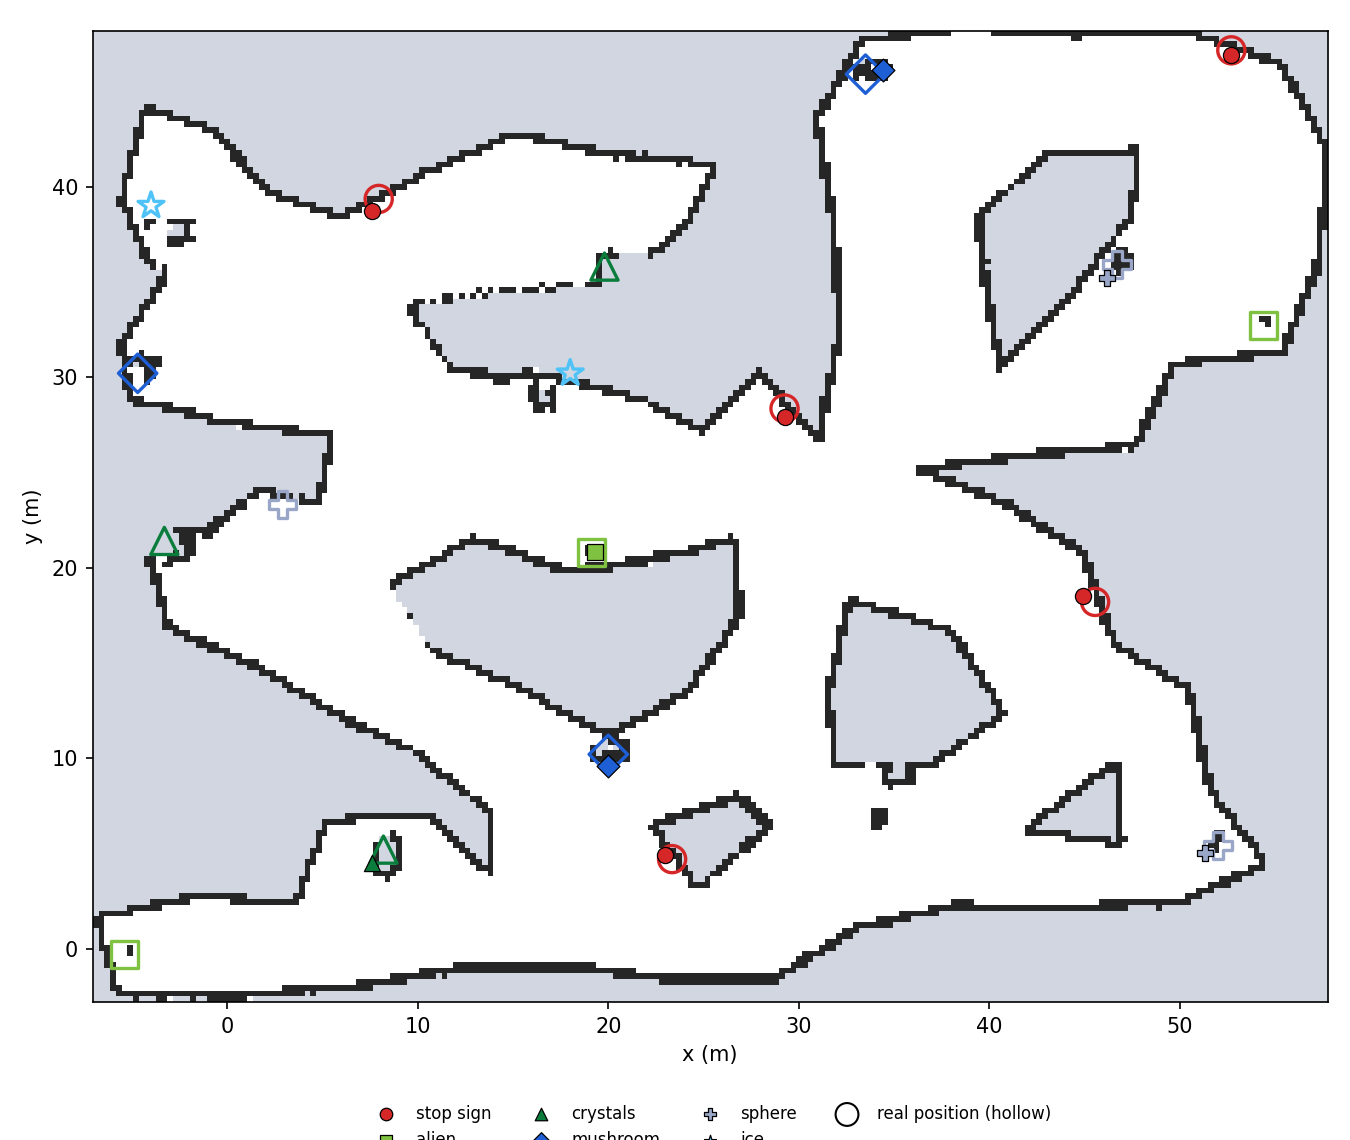
\includegraphics[width=0.62\linewidth]{perception3_markers.png}
  \caption{Placed artefact markers (filled) against the real positions from the world file (hollow) on the SLAM map after a 12-minute run. Ice detection was off.}
  \label{fig:p3map}
\end{figure}

\paragraph{Possible improvements.} Exploring for longer, or driving to unvisited artefacts, would place more of them. Artefacts beside a wall are seen from one side only, and the position error of crystals and ice
is mostly the size of the object. Using the depth over the whole box to estimate the object's centre, rather than its nearest surface, would reduce that error.


% =====================================================================
\section{Planning}
\label{sec:planning}
Exploration, inspection and behaviour switching run in one ROS~2 node (\texttt{cave\_explorer.py}), started by the autonomy
launch together with SLAM and Nav2. The node reads the occupancy grid from SLAM, chooses goals and sends them to Nav2 as
\texttt{NavigateToPose} actions. A main loop at 5\,Hz runs the state machine of Planning~3, and two 20\,Hz timers drive the
stuck recovery and the close-range confirmation of Planning~2. Goal choice and stuck detection are kept in \texttt{planning/safe\_navigation.py},
which has no ROS dependency and can be tested without the simulator.

\subsection{Planning 1 --- Autonomous exploration}
\paragraph{Method.} The node explores with frontiers: cells of known free space that border unknown space. Frontier cells are
grouped into connected clusters, and clusters shorter than five cells (about 1.5\,m) are ignored. For each cluster a goal is
searched within 3\,m of the frontier, in cells that are at least 1.2\,m from any wall or unknown cell, so that Nav2 is never asked
to drive into space it cannot see. The path length from the rover to every free cell is computed with Dijkstra's algorithm over the
occupancy grid (SciPy), the same method as the Dijkstra planner of Assignment~2 (Table~\ref{tab:prior}). Goals that cannot be
reached are discarded, and the remaining goal with the shortest path is chosen. Choosing by path length rather than straight-line
distance stops the rover from selecting a frontier that is close across a wall but far by road.

\paragraph{Start-up.} The rover first turns once on the spot through $360^\circ$ at 0.4\,rad/s, which takes about 25\,s, before it chooses a frontier. One alien stands
5.4\,m behind the spawn point, and a rover that drives away facing forwards never sees it. During the turn the detectors run as usual, and in a test the alien was placed at its true
position.

\paragraph{Failures and recovery.} A goal that fails is remembered, and no new goal is chosen within 3\,m of it. A goal that Nav2
aborts within 3\,s of receiving it is retried up to twice, and a goal that Nav2 rejects while it is still starting is sent again after 3\,s,
because Nav2 refuses a goal that arrives while it is finishing the previous one. A watchdog flags the rover as stuck when it moves less
than 0.5\,m in 15\,s. The goal is then cancelled and remembered as failed, and the rover reverses for 4\,s and turns for 2\,s before a
new goal is chosen. Exploration is treated as finished after 15 consecutive searches find no safe, reachable frontier.

\paragraph{Visualisation.} RViz shows the candidate goals (yellow spheres), the chosen goal (green sphere) and the failed goals
(red cylinders) on the SLAM map. The Detections image carries a line of text with the task the rover is doing, for example
``Exploring: driving to a frontier'' or ``Inspecting close up: moving closer''.

\paragraph{Limits and possible improvements.} Frontiers are ranked by path length only. Scoring them by the expected unknown area visible
from the goal would explore large chambers sooner. After exploration finishes, the rover stays where it is; returning to the start would
be a natural final step. The laser is mounted about 1\,m above the floor and does not see the low base of the crystal clusters, so the
planner can route the rover onto one. The stuck watchdog recovers from this in most cases, but in one of about five earlier runs the rover
stayed wedged on a crystal base.

\subsection{Planning 2 --- Close-range inspection}
\paragraph{Trigger.} The node inspects stop signs. A sign must be detected by the red-octagon classifier
(Section~\ref{sec:perception}) in two consecutive frames before it is acted on, which removes most single-frame false boxes. The
other artefact types are detected and placed on the map (Section~\ref{sec:p3}), but only stop signs are inspected at close range.

\paragraph{Placing the sign on the map.} The bearing of the sign comes from the column of the box centre and the camera's
$120^\circ$ horizontal field of view. Its range is the median of the nearest 30\,\% of depth readings inside the box, accepted
between 0.5 and 9.9\,m; the nearest readings are used because the box also contains rock behind the sign. For every correctly placed sign
in the captures, the box height in pixels multiplied by the range is between 390 and 500; a value outside 320 to 650 means the depth
was read from a wall in front of or behind the sign, and the sign is then treated as too far away to place. A sign seen beyond the depth
camera's 10\,m range cannot be placed either. The rover then drives along the sign's bearing to the farthest known-free cell within
12\,m that has 0.9\,m clearance, and places the sign once its depth can be measured. This approach is triggered at most once every
20\,s. A new position within 2\,m of a known artefact is treated as the same artefact.

\paragraph{Approach goal.} The inspection goal lies on the line from the rover to the artefact, 2.5\,m short of it, with the heading
set to face the artefact so that it stays in the camera's view. A closer stand-off was tried first, but a sign is tall and is cut off by
the edge of the image when the rover is nearer than about 2\,m. If the rover is already within 2.5\,m, the goal is a turn on the spot
towards the artefact. Nav2 plans and drives the path to the goal.

\paragraph{Close-range confirmation.} Arriving at the goal does not count as an inspection, because the sign may not be there: a
false sign placed from a distance looks the same to Nav2. A separate loop at 20\,Hz first turns the rover to face the artefact. If the
sign is seen but farther than 2.5\,m, the rover creeps forward at 0.25\,m/s, still facing it, for at most 6\,s. The inspection is accepted when
the sign is seen and measured within 3.5\,m, or when it was measured within 3.5\,m and then left the image because it no longer fits. If the
confirmation is not completed within 12\,s, the artefact is abandoned at once: going back to the same place would show the same thing.

\paragraph{Difficulties.} The first versions placed signs at a fixed 3\,m along the bearing, which put distant signs at the wrong
position and sent the rover to empty rock. Measuring the range with the depth camera, and using the true field of view of the
camera, removed most of these errors. The depth of a sign near a wall could still come from the wall, which produced a second, false
artefact and sent the rover into a corner; the size check on the box above removes this. Nav2 reports arrival within about a metre
of the goal, so before the confirmation was added, a sign that was out of view at the goal still counted as inspected.

\subsection{Planning 3 --- Behaviour switching}
\paragraph{State machine.} The node has four states. In \textsc{explore} it chooses and follows frontier goals. When a new artefact
is placed, it switches to \textsc{preempt}: the frontier goal is cancelled, and the node waits until Nav2 has released it. It then
switches to \textsc{inspect} and sends the approach goal of Planning~2. When the inspection goal succeeds it switches to \textsc{confirm}, the
close-range confirmation. When that is accepted the artefact is recorded as inspected and the node returns to \textsc{explore}.

\paragraph{Timeout, retry and abandon.} An inspection fails when Nav2 reports a failure, when the approach takes longer than its
limit, when the artefact is out of sight, or when the rover is stuck on the way. The time limit is 20\,s plus 4\,s per metre of the
approach, up to 90\,s, with a new clock for each artefact. The artefact counts as out of sight only while the rover is facing it, within
$50^\circ$ of its heading and nearer than 9\,m, for more than 8\,s, because a sign behind a corner is not lost. If the rover has moved
less than 0.5\,m in 15\,s and is more than 1\,m from the approach point, the goal is cancelled and the rover backs up. On the first failure
the approach goal is recomputed and sent again. On the second failure, or as soon as the sign is not seen at close range, the artefact is
recorded as abandoned and the node returns to exploration.

\paragraph{Visited record.} Every artefact is kept in a list with its position and status: pending, inspected or abandoned. A
detection within 2\,m of an artefact already in the list is ignored, so no artefact is inspected twice and an abandoned artefact is
not retried. RViz shows the status of each artefact as a coloured sphere: yellow for pending, green for inspected and red for
abandoned.

\paragraph{Difficulties.} Cancelling a goal and sending the next one overlap in time: the result of the cancelled goal can arrive
after the new goal has been sent and be mistaken for its result. Each goal therefore carries a generation number, and a result is
used only if it belongs to the current goal. The state machine also waits in \textsc{preempt} until Nav2 has released the frontier
goal, because a new goal sent before then is rejected. The start time of an inspection was at first not reset between artefacts, so
each new artefact inherited the previous one's clock, timed out at once and used up its retry; the clock now starts when the approach goal
is sent.

\paragraph{Possible improvements.} A sign seen from two places can be placed twice more than 2\,m apart and then be inspected twice.
These duplicates could be merged once the rover is close enough to measure both. Inspection could be extended to the alien, crystals,
mushroom and sphere, which are already detected and placed on the map.

\subsection{Results of the finished node}
\label{sec:integration}
Table~\ref{tab:final} gives two 12-minute runs of the finished node in Gazebo, on the same cave, each started from a fresh simulator
with the code as submitted. Figure~\ref{fig:final} shows the mapping progress and the path of each run.

\begin{table}[h]
\centering
\caption{Two 12-minute Gazebo runs of the finished node, on the same cave map, each started from a fresh simulator. Run 2 is the code as submitted; Run 1 has the same planning code, from before the image saving and the launch-file change were added. Counts come from the node logs and the position recorder.}
\label{tab:final}
\begin{tabular}{@{}lcc@{}}
\toprule
 & \textbf{Run 1} & \textbf{Run 2} \\
\midrule
Real stop signs inspected (of 5)                  & 5 & 5 \\
Artefacts reported                                & 6 & 6 \\
Artefacts not near a real stop sign               & 0 & 0 \\
Inspections completed                             & 6 & 6 \\
Inspections that timed out                        & 0 & 0 \\
Stuck events handled                              & 0 & 1 \\
Frontier goals chosen                             & 21 & 22 \\
Goals that failed or were cancelled               & 4 & 5 \\
Distance driven [m]                               & 207 & 227 \\
Cave mapped at the end [\%]                       & 100 & 100 \\
Robot stops moving at [s]                         & 305 & 360 \\
Manual rescues needed                             & 0 & 0 \\
\bottomrule
\end{tabular}
\end{table}

\begin{figure}[h]
  \centering
  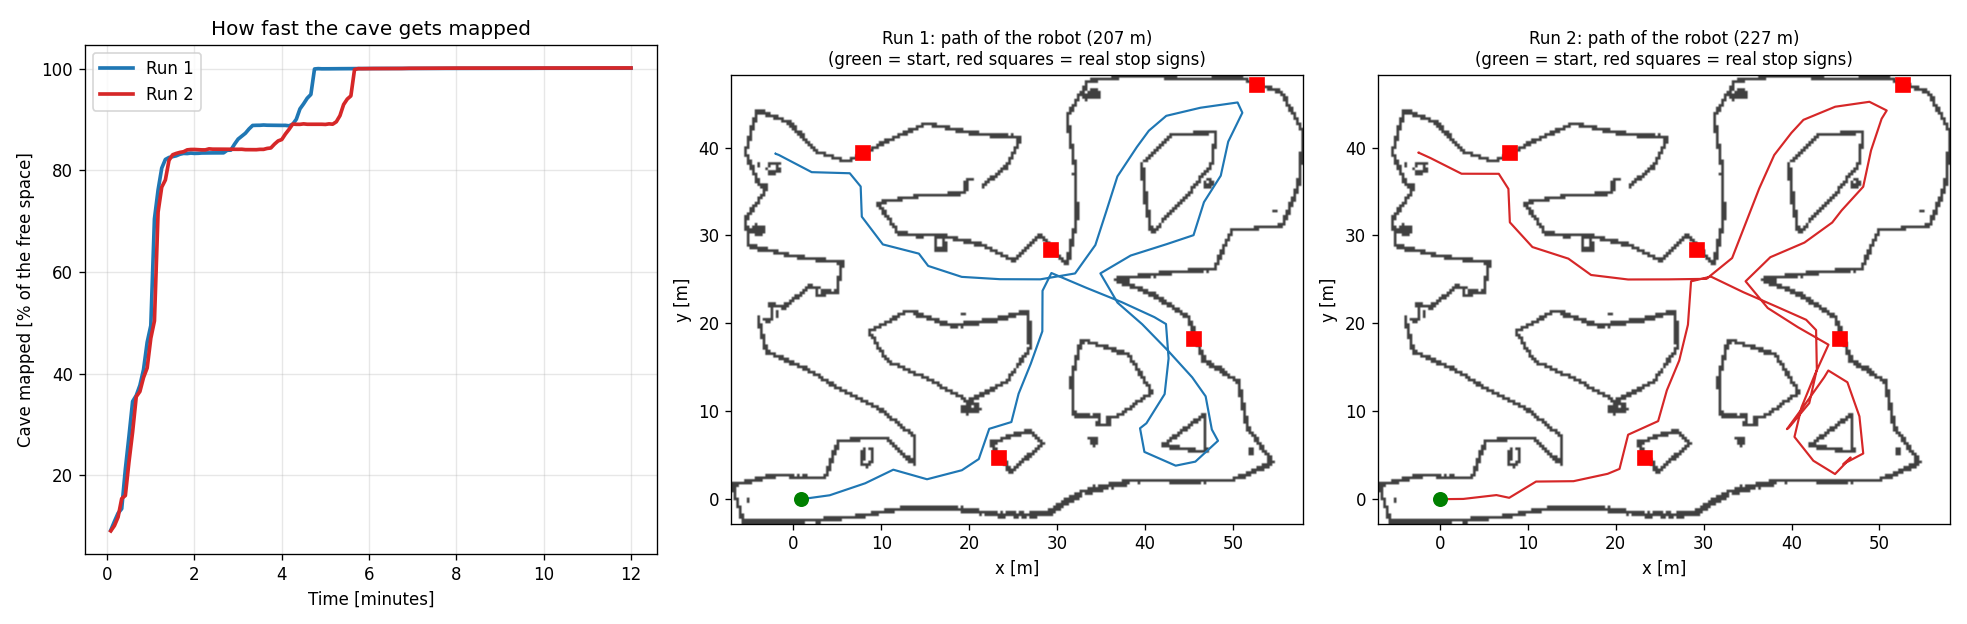
\includegraphics[width=0.85\linewidth]{planning_final_runs.png}
  \caption{Left: share of the cave's free space mapped over time. Middle and right: path of each run (red squares: real stop signs).}
  \label{fig:final}
\end{figure}

\paragraph{Reading the results.}
In Table~\ref{tab:final}, all five stop signs were inspected in both runs, and each was confirmed close up at 2.4 to 3.2\,m. Neither run had an inspection time out. Run 2 had one stuck
event on a frontier goal, which the watchdog cleared without help. The cave was fully mapped in both runs, and the robot stopped moving 5 to 6 minutes in, when no frontier was left to explore.
Six artefacts were reported for the five signs: in both runs one sign was placed twice, more than 2\,m apart, from two viewpoints, and was inspected twice. All six artefacts were within 6\,m of a real sign.
Real sign positions come from the world file and are used only to check the results; the code never uses them. Two runs is a small sample,
so these figures describe the behaviour seen in these runs and are not a measured success rate. Earlier versions of the node, before the
timeout, confirmation and size-check changes, had two inspection timeouts and two or three inspection goals away from any real sign per run.

% =====================================================================

% =====================================================================
\section{Advanced 2 --- Cave Geometry Analysis}
\label{sec:advanced2}

\subsection{What the task asks for}
As the rover explores, the program should work out the \emph{shape} of the cave from the map the rover is
building. In particular it should find the \textbf{widest open area} found so far and a \textbf{narrow passage}
(a bottleneck), and show both in RViz on top of the map. Wide areas could suit future human activity, and narrow
passages matter for navigation and safety. The result is updated every time the map changes.

\subsection{The idea in one picture}
\label{sec:a2idea}
The method rests on one simple question, asked for every free spot on the map:
\emph{how far away is the nearest wall?} Everything else (the centre-line, the widest area, the narrow spots)
is read off the answer. Figure~\ref{fig:a2steps} shows the six steps on the real map from a Gazebo run, and the text
below explains each one.

\begin{figure}[h]
  \centering
  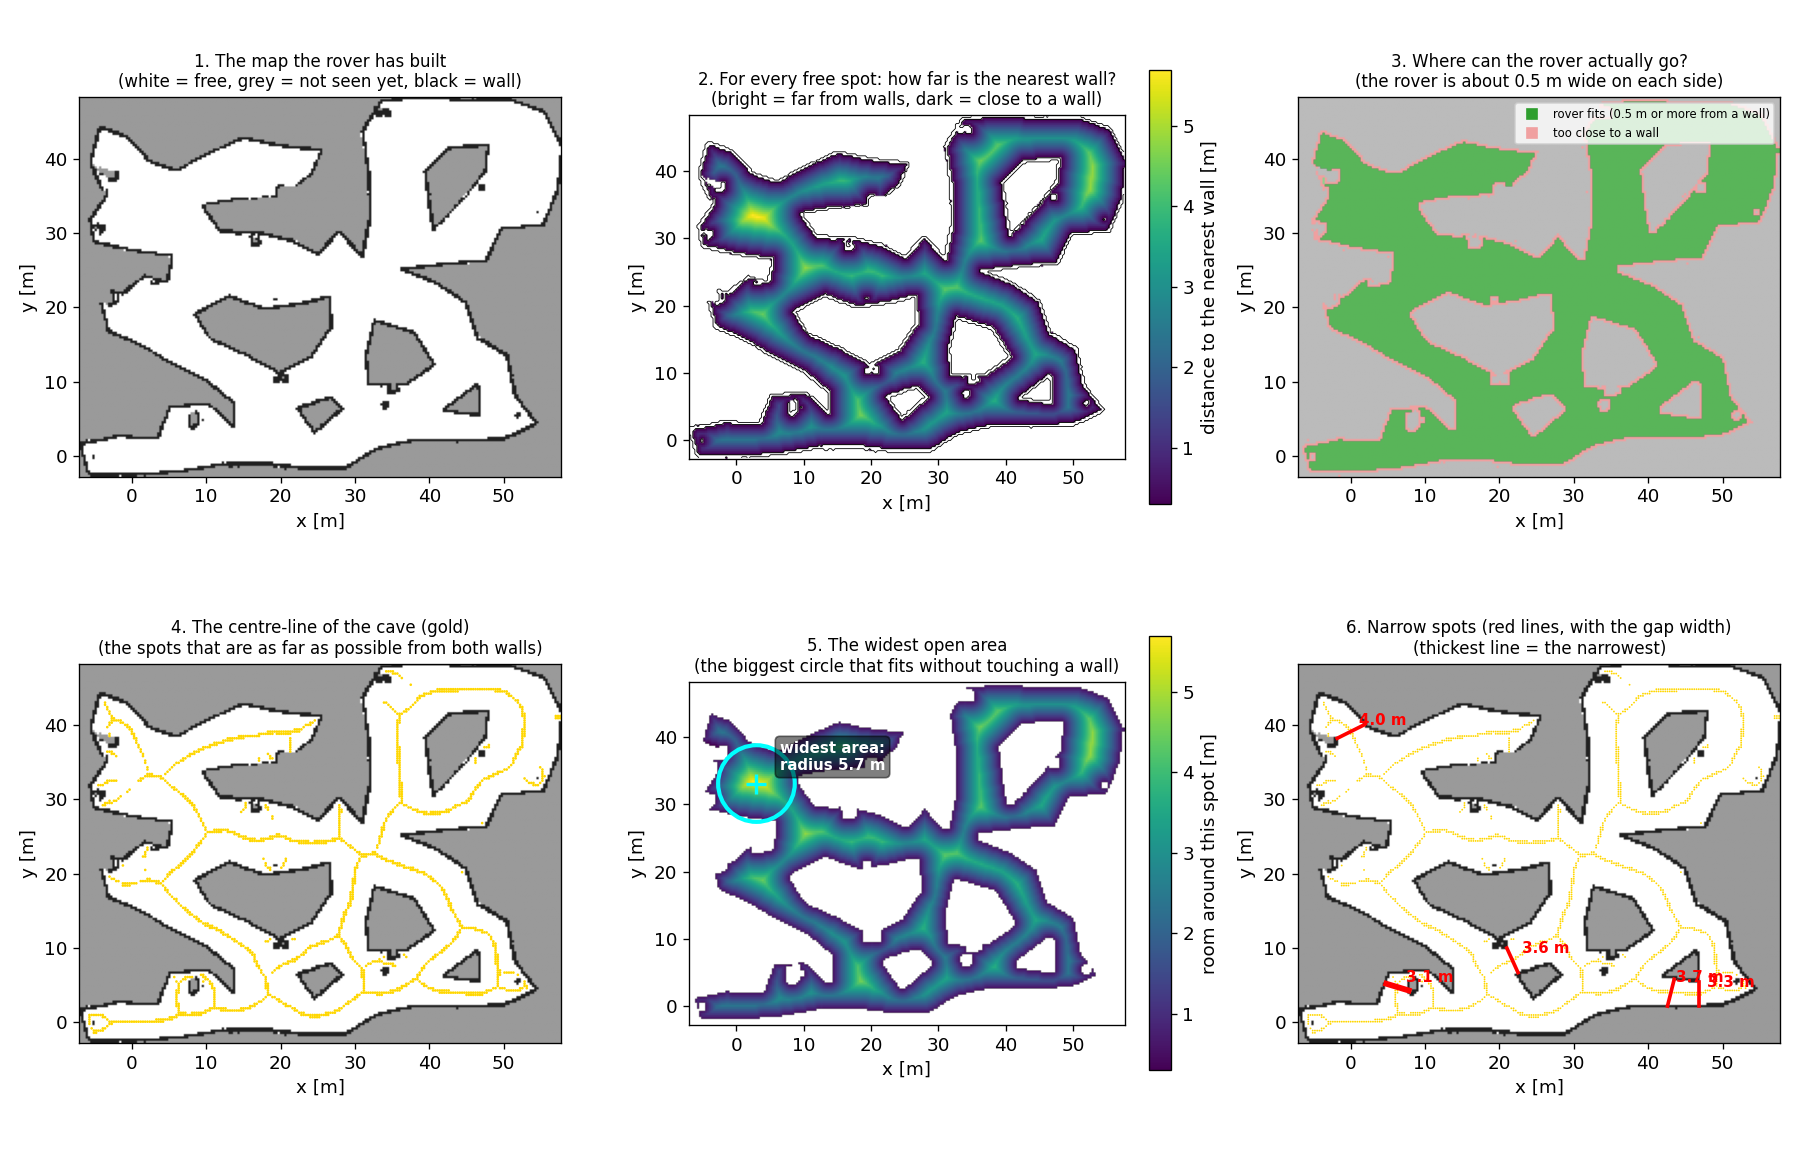
\includegraphics[width=0.85\linewidth]{advanced2_steps.png}
  \caption{The six steps of the cave geometry analysis, on the map the rover built in Gazebo.}
  \label{fig:a2steps}
\end{figure}

\begin{enumerate}[nosep]
  \item \textbf{The map.} The rover's map is a grid of small squares, each 0.3\,m wide. Every square is marked
        as free, as a wall, or as not seen yet. Only cells the rover has observed are used.
  \item \textbf{Distance to the nearest wall.} For every free square the program works out how far it is from the
        closest wall. Squares in the middle of a wide room get large numbers, and squares hugging a wall get small
        ones. (The technical name for this is a \emph{distance transform}. It is the quantity from Task~9 of Assignment~2, computed here with an exact Euclidean transform.) It is recalculated whenever the map
        updates, so it grows with the map.
  \item \textbf{Where the rover can go.} The rover is about 0.5\,m wide on each side, so squares closer than 0.5\,m to a wall are
        ruled out, and so are free areas the rover could not reach from where it is.
  \item \textbf{The centre-line.} Consider walking away from a wall. The distance to it grows by exactly one metre
        for each metre you walk. That stops being true on the centre-line of a corridor: step towards one wall and
        you move away from the other, so the distance stops growing steadily. The program looks for exactly the spots where the
        distance stops growing steadily and marks them in gold. They form a line along the middle of every
        passage. (The technical name is the \emph{medial axis}. The rule uses how fast the distance changes from
        square to square, its \emph{gradient}.)
  \item \textbf{The widest open area.} Among all the squares the rover can reach, the program finds the one with the most
        room around it. The circle that just fits there, touching no wall and no unseen space, is the widest open area,
        and its radius says how roomy it is. Unseen space is not counted as open.
  \item \textbf{Narrow spots.} A narrow spot is a place along the centre-line where the gap between the walls is
        smaller than nearby, like a doorway between two rooms. Each one is shown as a red line across the gap, labelled with
        the width. The thickest line is the narrowest. Each candidate must pass a verification test, described next.
\end{enumerate}

\begin{lstlisting}[caption={Step 4 in code: the centre-line is where the distance stops growing by one metre per metre.}]
def ridge_of(clearance, accessible, resolution, gradient_threshold=0.8):
    d_row, d_col = np.gradient(clearance, resolution)
    return accessible & (np.hypot(d_row, d_col) < gradient_threshold)
\end{lstlisting}

\subsection{How a narrow spot is tested}
\label{sec:a2cut}
A spot on the centre-line where the gap is small is only a \emph{narrow passage} if it divides the free space.
A small bump on a wall also makes the gap smaller, but it divides nothing. So each candidate gets a
\emph{cut test}: draw a line across the gap, from the nearest wall on one side to the nearest wall on the other, and treat the
line as a wall. Then look at the free space around it (within 5\,m). If it splits into two separate areas,
each at least 3\,m$^2$, and at least one of them opens out to 1.5 times the gap, it counts as a narrow passage.
Figure~\ref{fig:a2cut} shows one candidate that passes the test and one that fails.

\begin{figure}[h]
  \centering
  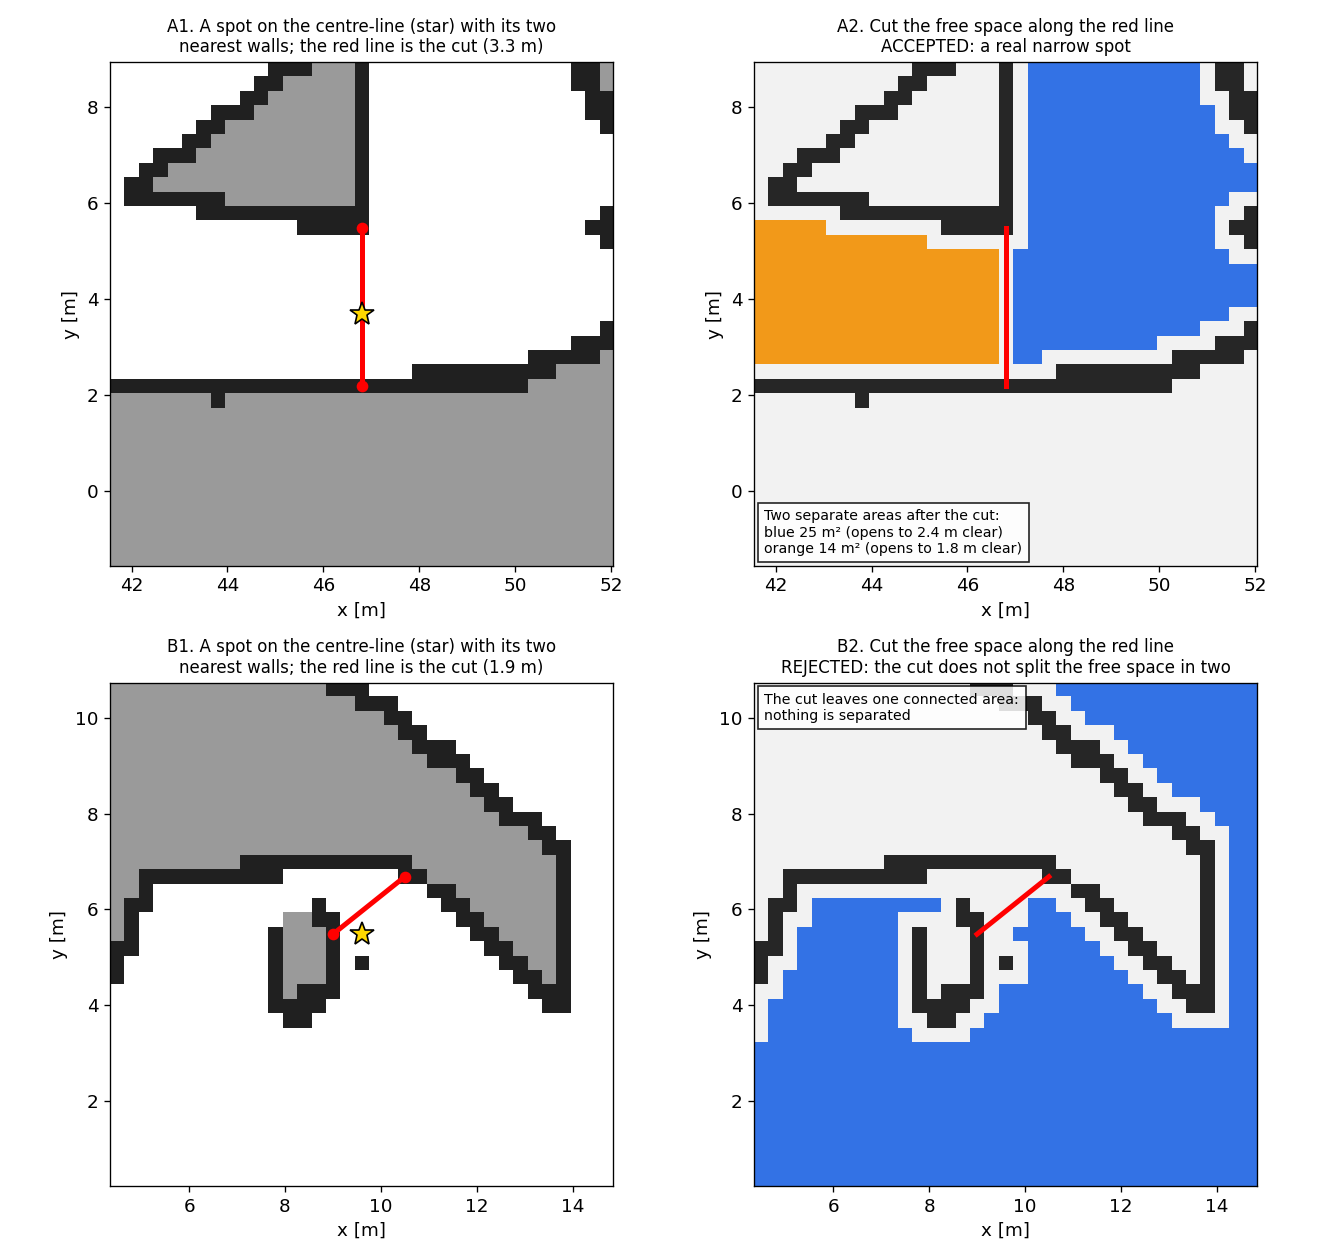
\includegraphics[width=0.75\linewidth]{advanced2_cut_test.png}
  \caption{The cut test. Top: a 3.3\,m gap, where cutting along the red line splits the free space into two separate
  areas (blue and orange), so it is accepted. Bottom: a small bump in a wall, where the cut leaves one connected area,
  so it is rejected.}
  \label{fig:a2cut}
\end{figure}

Two further details. Each passage is called a \emph{doorway} if both sides open out and a \emph{corridor} if only one
does. The program also checks whether the spot is a \emph{saddle}, like a mountain pass between two wider areas, using the
curvature of the distance map. This is reported but not used to decide.

\paragraph{Stabilising the reported result.}
The map moves by one square between updates. Early on, this made the ``narrowest passage'' jump between
near-equal candidates 31 times in one run. A passage is now shown only if it was also found, within 1.5\,m, in the
previous update, and a change is announced only if the width moves by more than 0.5\,m or the place by more than
3\,m. A short-lived false 1.2\,m doorway, caused by a partly mapped wall, disappeared with this check.

\subsection{The data going in and out}
\label{sec:a2data}
The program reads the SLAM map from \texttt{/map} about every 2\,s (one number per 0.3\,m square: $-1$ not seen, 0 free, 100 wall; the map in Figure~\ref{fig:a2slam} is $216\times170$ squares). It publishes the distance to the nearest wall as a grid of the same size, and RViz markers: gold dots for the centre-line, a cyan disc and label for the widest area, and red and orange lines with width labels for narrow spots. Changes to the widest area and the narrowest passage are also printed in the terminal.


\subsection{Results}
\label{sec:a2results}

\paragraph{On the map the rover built.}
The same analysis was run on the map made by \texttt{slam\_toolbox} during a full Gazebo run
(Figure~\ref{fig:a2slam}). It found a reachable area of about 1500\,m$^2$, the widest open area with a radius of
5.7\,m at $(3.0, 33.1)$ (about 100\,m$^2$), and five narrow spots, 3.1, 3.3, 3.6, 3.7 and 4.0\,m wide. The widest
area is the large chamber in the top left of the map.

\begin{figure}[h]
  \centering
  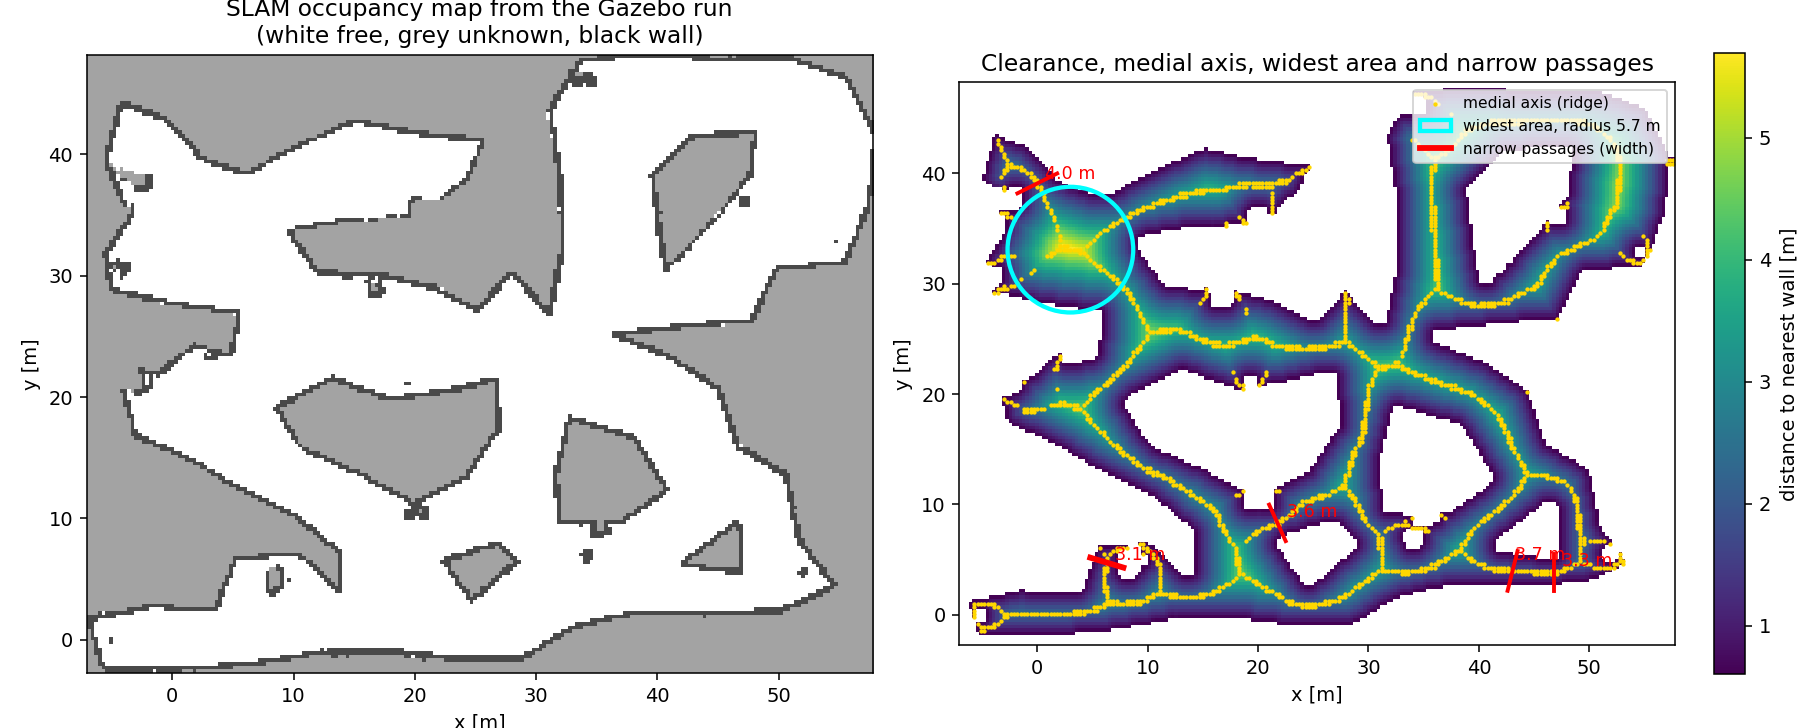
\includegraphics[width=0.85\linewidth]{advanced2_gazebo_slam_geometry.png}
  \caption{The final result on the real map from a Gazebo run. Right: gold is the centre-line, the cyan circle is
  the widest open area, and red lines are narrow spots with their widths.}
  \label{fig:a2slam}
\end{figure}

\paragraph{It grows as the rover explores.}
In a replay of the Gazebo run of Figure~\ref{fig:a2slam}, the map is shown only around the places the rover had visited so far (within
12\,m of each stop), then analysed. After the first stop, the widest area has a radius of 2.8\,m. After three stops it is 4.5\,m,
and after eight it reaches 5.7\,m, when the rover reaches the big chamber in the top left. The known free space grows from 82\,m$^2$ to more than
1000\,m$^2$ over the same stops.


\paragraph{Checking against a separate source.}
To check the answer is sensible, the same analysis was run on a map drawn directly from the wall positions in the
simulator's world file, with no simulator running. This is independent of the laser and of SLAM.


The widest area agrees within 0.2\,m in radius and 0.7\,m in position. Both maps find the same two gaps of about
3.1--3.3\,m, near $(6,4)$ and $(47,4)$, but they disagree about which is narrowest. The difference is 0.2\,m or less,
which is smaller than one map square (0.3\,m), so it is not meaningful. The gap near $(6,4)$ is missing from the
world-file map. A likely reason is that the real laser also sees the green crystals standing beside it, which the
wall-only drawing leaves out.

\paragraph{Speed.}
On the whole cave, one analysis takes about 0.02\,s, so it keeps up with map updates.


\begin{figure}[h]
  \centering
  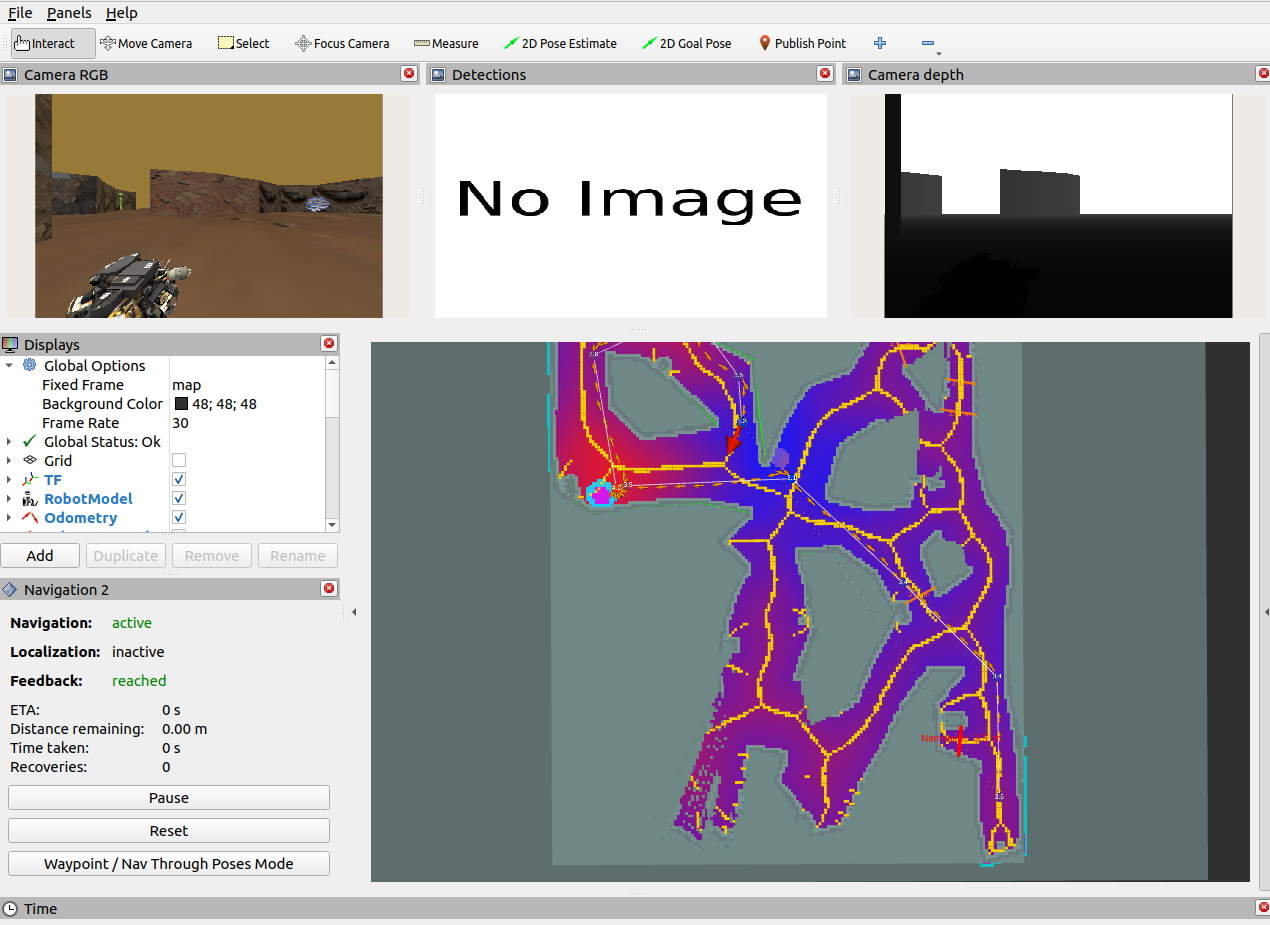
\includegraphics[width=0.7\linewidth]{rviz_run_screenshot.png}
  \caption{RViz during a Gazebo run (screenshot taken while the first, 10-reading run was in progress). The map panel shows the
  cave geometry overlay: the colour shows the distance to the nearest wall (red = the most room, as in the large chamber at the
  top left, blue = close to walls), the gold lines are the centre-line, the cyan disc is the widest open area, and the red line and label near the bottom right mark the narrowest
  passage (other narrow passages are orange). The white lines join the sampling spots in the order visited, with the readings written beside them (Advanced~6). The
  Detections panel is empty because the node that fills it was not running in this test.}
  \label{fig:rviz}
\end{figure}

\subsection{Limits and possible improvements}
\begin{itemize}[nosep]
  \item The cave is 3--5\,m wide throughout, so ``narrow'' is relative. A gap is only judged narrow compared with the space beside it.
  \item Widths are only as exact as the map squares (0.3\,m), so close results cannot be ranked reliably.
  \item A long corridor of constant width is reported at its mouth, not along its length.
  \item The analysis is not yet used by other parts. It could, for example, choose where to place sensors or relays, or serve as the
        skeleton of a roadmap (Advanced 4).
\end{itemize}

% =====================================================================
\section{Advanced 6 --- Adaptive Scientific Sampling}
\label{sec:advanced6}

\subsection{Objective}
Let the rover measure a spatially varying science quantity at its position, build a Gaussian Process
(GP) model of the field from its own measurements, use the prediction and its uncertainty to choose
where to sample next, and compare this with a simple baseline. The sampler must not use the true field
when choosing.

\subsection{The science data: real NASA measurements of water in Martian soil}
\label{sec:nasadata}

\paragraph{What it is.}
To make the task realistic, the field is based on real measurements rather than an invented pattern. The measurements were taken by NASA's
\emph{2001 Mars Odyssey} satellite, which has orbited Mars since 2001. One of its instruments, the
\emph{Gamma Ray Spectrometer}, detects the faint gamma rays that the ground gives off. Water changes this signal,
so scientists can work out how much water is mixed into the top layer of the soil. The result is a map of
Mars showing how wet the soil is in each place. We downloaded it from NASA's public Planetary Data System
(data set \texttt{ODY-M-GRS-5-ELEMENTS-V1.0}, file \texttt{H2O\_SR\_5X5}; measurements made between June 2002
and April 2005)~\cite{pds}. The way the values were derived is described in the paper by
Boynton and colleagues~\cite{boynton2007}.

\paragraph{How the amount of water is written.}
The amount is given as a \emph{percentage of the soil's weight}. A value of 4 means that 4\,kg of every 100\,kg of
soil is water. Over the whole planet the values run from 1.6 to 7.4. In the block used here, they run from 2.3 to 5.0.

\paragraph{What is in the file.}
NASA split the planet into a grid of squares, each $5^{\circ}$ of latitude by $5^{\circ}$ of longitude
(about 300\,km on each side). The file has 2592 squares, and each square is one line with five numbers.
1508 squares have a measurement. The rest, near the poles, are marked with the code 9999.999, meaning ``no data''.


\subsection{How the data was put onto the cave map}
\label{sec:nasaonmap}

The rover explores a cave about $65 \times 55$\,m, so the NASA map had to be fitted onto it. This was done in
five steps. The same steps are in the software, in \texttt{measurement\_field.py}.

\begin{enumerate}[nosep]
  \item \textbf{Choose a piece of Mars.} We took a block of $12 \times 12 = 144$ squares around Arsia Mons
        (latitude $37.5^{\circ}$S to $17.5^{\circ}$N, longitude $212.5^{\circ}$ to $267.5^{\circ}$E).
        Arsia Mons is a giant volcano, the southernmost of three in a row on the Tharsis bulge, a large raised region
        near the equator of Mars. It lies at $8.35^{\circ}$S, $239.91^{\circ}$E~\cite{wiki_arsia}, close to the middle of the
        block. We chose it because every square has a measurement, because the
        water varies from place to place (so there is something to discover), and because the water values vary across the block.
  \item \textbf{Match it to the map.} The cave map uses metres: $x$ runs from $-5$ to $60$ and $y$ from
        $-5$ to $50$. We stretched the block of Mars over this rectangle in a straight, even way:
        \begin{equation*}
          \text{longitude} = 212.5 + \frac{x+5}{65}\times 55, \qquad \text{latitude} = -37.5 + \frac{y+5}{55}\times 55 \;=\; y - 32.5 .
        \end{equation*}
        For example, the rover's start $(x,y)=(0,0)$ is placed at $32.5^{\circ}$S, $216.7^{\circ}$E. A position outside
        the rectangle uses the nearest edge.
  \item \textbf{Make it smooth.} A square has a single number, but the rover can stand anywhere. Between the
        middles of neighbouring squares we blend the numbers in a straight line, so the water changes smoothly
        and has no sudden steps.
  \item \textbf{Give each place its true value.} Now every position the rover can reach on the map has a
        \emph{true} water value. This is kept hidden from the part of the program that decides where to go.
  \item \textbf{Make readings imperfect.} A real instrument is never exact. When the rover takes a reading, the
        program returns the true value plus a small random error of the size NASA reports for that square (0.23 to
        0.36 inside our block, 0.27 on average). Two readings at the same place therefore differ slightly.
\end{enumerate}

\begin{figure}[h]
  \centering
  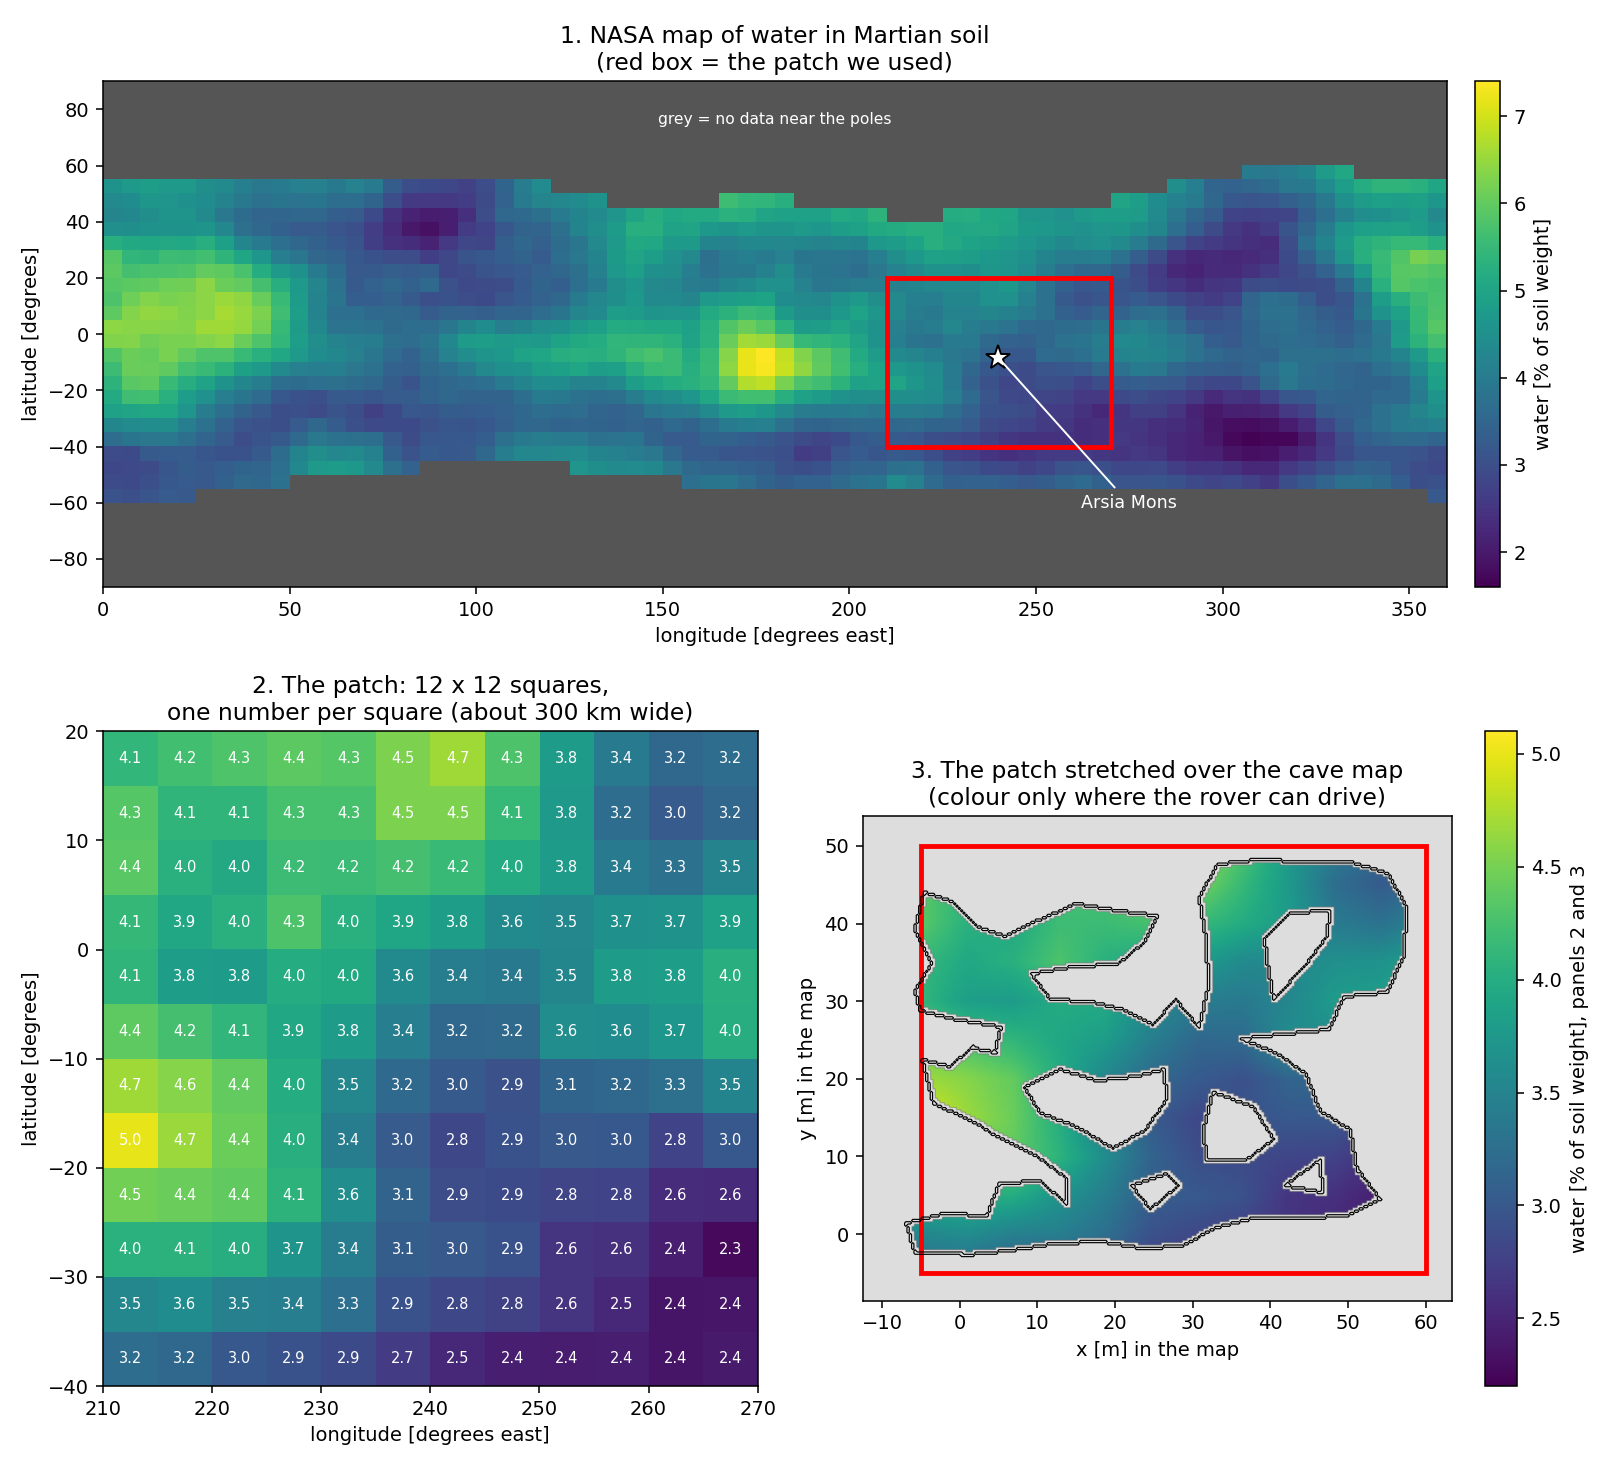
\includegraphics[width=0.8\linewidth]{advanced6_nasa_field_on_map.png}
  \caption{From NASA's map to the cave map. (1)~The whole NASA map of water in Martian soil; the red box is the
  block we used, and the star marks Arsia Mons, a giant volcano near the middle of the block. (2)~The block itself: 144 squares with their values. (3)~The same block
  stretched over the cave map. Colour is shown only where the rover can drive. Panels 2 and 3 share one colour scale.}
\end{figure}

\paragraph{The scale is not realistic.}
One square on Mars is about 300\,km across, and our block is about 3250\,km wide, roughly the distance from Sydney
to Perth. The whole block is compressed into a cave tens of metres wide, so one metre in the cave stands for about 50 to
60\,km on Mars. The task does not need the numbers to match a real cave, only a believable field that varies from
place to place.

\paragraph{Where the data is in the simulator.}
The water values are not objects that you can see in Gazebo's 3D view. They exist inside the software as a lookup:
the program is given a position on the map and returns the water value there. They are drawn for people in RViz,
on the same map the rover is building (Section~\ref{sec:a6example}). Each square's latitude and longitude give its place on the cave map in metres, its concentration is the true water value there (hidden from the rover when it chooses where to go), and its error sets the size of the random error added to each reading; the chosen block has no ``no data'' squares.


\subsection{What the data looks like in a simulator run}
\label{sec:a6example}

Figure~\ref{fig:a6run} comes from one real run in Gazebo: the rover took 30 readings with real navigation.
The first panel shows the 30 places it visited, in order, on top of the true field. The second shows what the rover
worked out about the whole cave from only those 30 readings. The third shows how unsure it still is. The fourth
compares each reading with the true value at that spot. The points lie close to the dashed line, so the readings
are close to the truth. The average mistake was $-0.03$ and the typical size of a mistake was $0.21$, which matches
the instrument error that NASA lists for this block (0.23 to 0.36). The rover's overall picture of the cave
(panel~2) was off by 0.23 on average. The brightest part of panel~3, in the top left of the cave, is the area
the rover has measured least.

\begin{figure}[h]
  \centering
  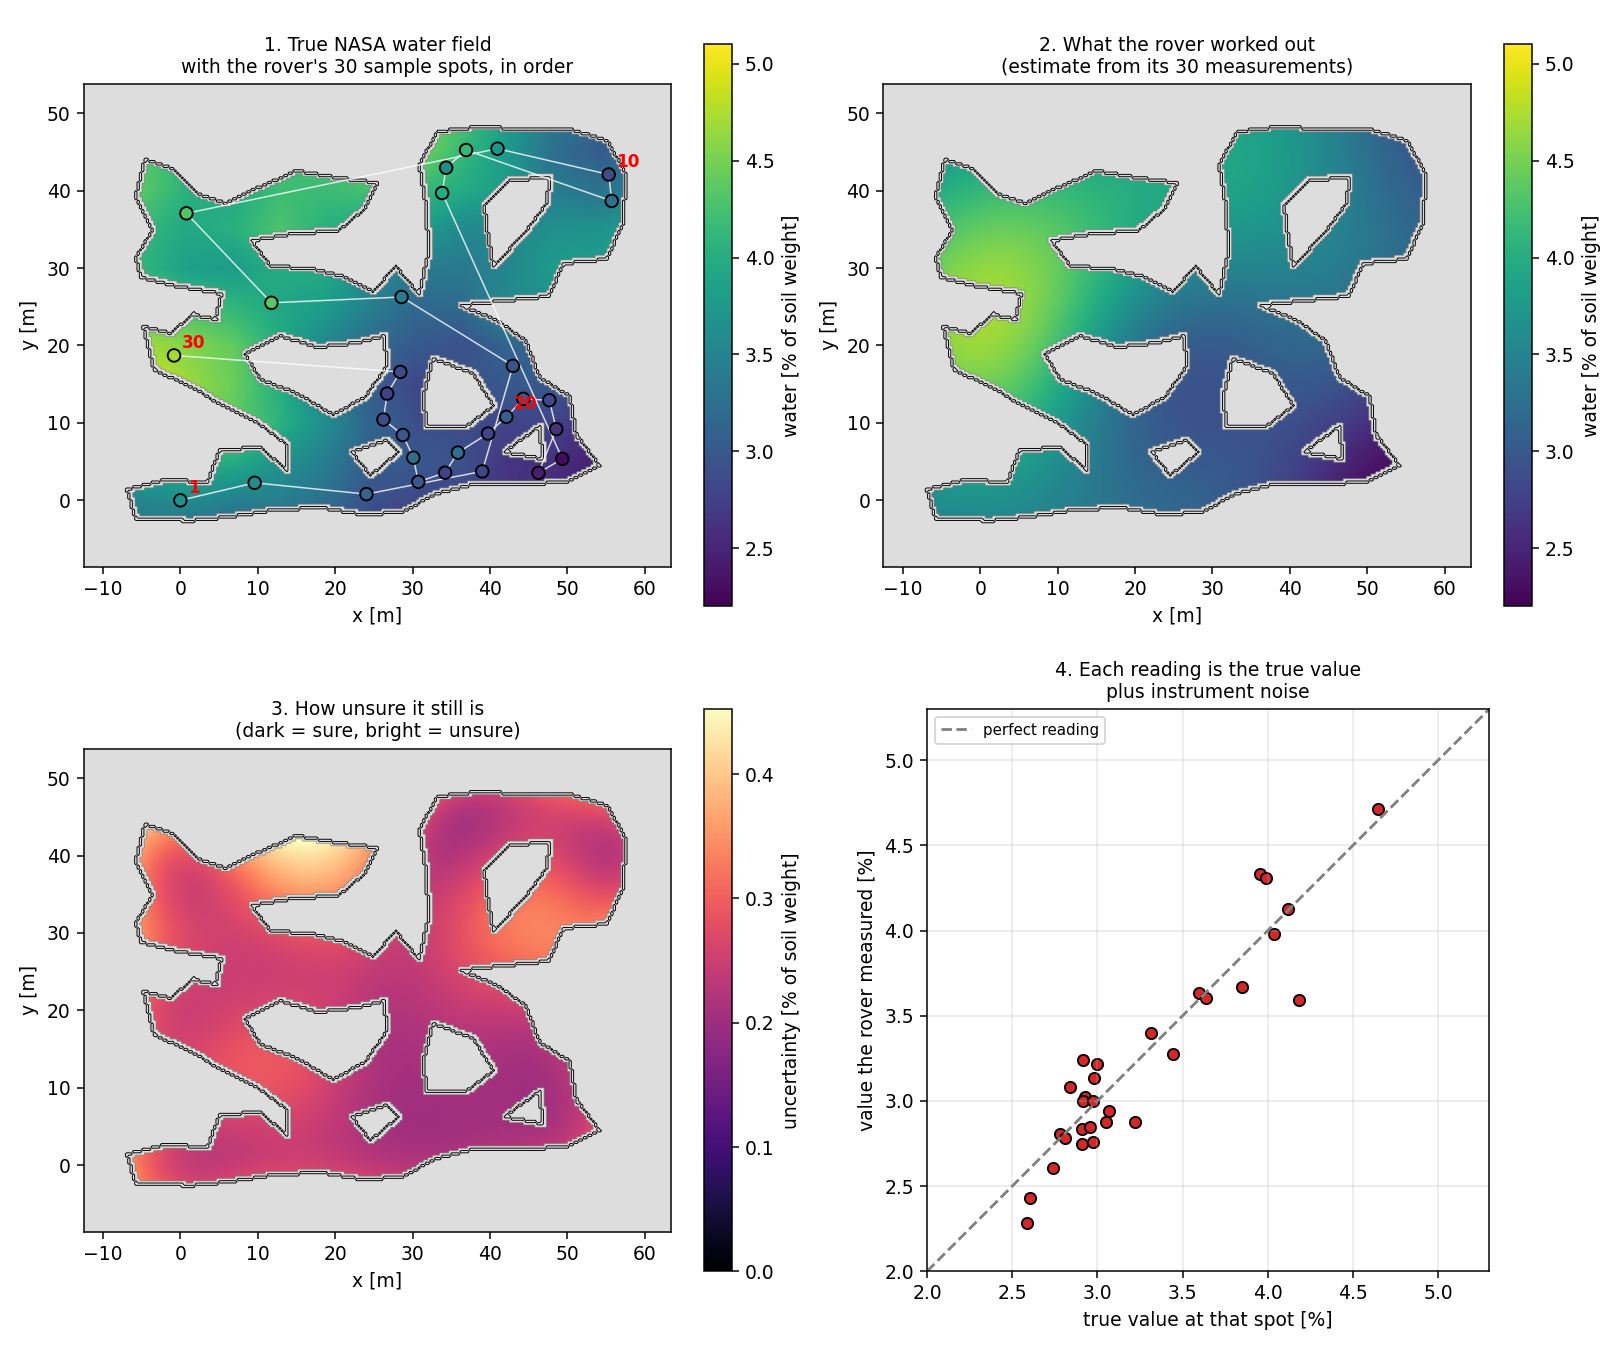
\includegraphics[width=0.85\linewidth]{advanced6_gazebo_run_maps.png}
  \caption{One 30-reading run in Gazebo. (1)~True field, with the places the rover measured, in order. (2)~The rover's
  estimate. (3)~Its remaining uncertainty. (4)~Each reading against the true value. The estimate was re-computed from
  the readings saved by the run.}
  \label{fig:a6run}
\end{figure}


\subsection{The real instrument and our virtual one}
\label{sec:instrument}

\paragraph{The real instrument.}
The water map was made by the \emph{Gamma Ray Spectrometer} on Mars Odyssey, a satellite that has circled Mars in a nearly circular orbit
about 400\,km above the surface~\cite{pds_catalog}. It is in fact a set of three instruments that work together: a gamma-ray
spectrometer, a neutron spectrometer and a high-energy neutron detector~\cite{boynton2004}. They cannot see water directly. Cosmic rays from
space hit the ground and knock out neutrons, and those neutrons make the soil give off gamma rays whose energies are a fingerprint of the
elements present. Hydrogen leaves a clear mark, and because most hydrogen on Mars is locked in water, scientists turn the hydrogen
signal into a water amount~\cite{feldman2004}. The instruments sense only the top layer of the ground, the upper few tens of centimetres~\cite{pds_catalog}.
From orbit, one measurement covers an area hundreds of kilometres across, which is why NASA's file uses squares 300\,km wide.

\paragraph{What was built instead.}
We did not simulate the detector, the gamma rays or the neutrons. We simulated what a user of the instrument gets out of
it: a water value, with an error, for a place. The rover gives its position, the program looks up NASA's water value
for that place (blending smoothly between squares), adds a random error of the size NASA reports for that square, and
returns the answer. In the code this is the function \texttt{measure(x, y)} in \texttt{measurement\_field.py}. The part of the
program that chooses where to go can call only this function, and never sees the true value.


\paragraph{What the simulation leaves out.}
It leaves out the physics of the gamma rays and neutrons, the blurring caused by the 300\,km footprint (ours reads a single point), and
any error that is shared between measurements. Our errors are all random and independent of each other, but real errors are partly
systematic. The nearest real equivalent for a rover is the neutron instrument on the Curiosity rover, called DAN, which looks for
hydrogen under the wheels~\cite{mitrofanov2012}. We did not model it.

\subsection{What is real and what is not}

\begin{table}[h]
\centering
\caption{Which parts of the data are real, which we adapted, and which are not real.}
\small
\begin{tabular}{@{}p{2.6cm}p{11.4cm}@{}}
\toprule
\textbf{Real} & The water values, where Mars is wetter and drier, and the size of the instrument's error. All of these come from NASA's file. \\[3pt]
\textbf{Adapted for this project} & The choice of block; stretching it over the cave; blending smoothly between squares; adding a random error to each reading (the size of the error is NASA's, the random numbers are generated by the computer). \\[3pt]
\textbf{Not real} & That the water in a cave would vary like this; the scale (one metre stands for 50--60\,km); and the idea that the rover has a water instrument at all. Also, NASA's file does not say whether longitude counts east or west. We assumed east, after checking that the known wet regions appear in the expected places. \\
\bottomrule
\end{tabular}
\end{table}

The task description allows this: it asks for a field that ``does not need to realistically match the cave environment''
as long as it gives a believable, varying quantity to measure.

\subsection{Method}
\paragraph{Separation of truth.}
The sampler (\texttt{adaptive\_sampling.py}) has no reference to the field. It receives one
measurement at a time. The true field is read in one place, to score the result.

\paragraph{Gaussian Process.}
scikit-learn's \texttt{GaussianProcessRegressor}, input the robot's $(x,y)$, a constant $\times$ RBF
kernel plus a white-noise term, targets normalised. The length scale is bounded to 5--60\,m. The
hyperparameters are fitted only from 8 samples; before that the prior (length scale 10\,m) is used, because
the fit on fewer samples chose a very short length scale that made everywhere look equally uncertain.

\paragraph{Choosing the next location.}
Candidates are cells of a 1\,m lattice in the accessible part of the current map, at least 1.5\,m from
walls and unknown space (so Nav2 can reach them), at least 4\,m from existing samples and at least 4\,m from
goals that failed. Each is scored by
\begin{equation}
  \text{score} = \frac{\sigma(\mathbf{x})}{\max\sigma} \;-\; w\,\frac{\text{path}(\mathbf{x})}{\max\text{path}},
\end{equation}
the GP standard deviation minus a penalty for the shortest path through free space (Dijkstra's algorithm on the
grid, as in Assignment~2, not straight-line distance). The best score is the next goal. The weight $w$ is the
\emph{travel weight}; 0.3 is the default and 0.1 was also tested. The baseline picks uniformly at random
from the same candidates. Because candidates exist only in the known map, the method also drives
exploration toward its edge.

\begin{lstlisting}[caption={Choice of the next sampling location (adaptive strategy).}]
_, std = self.predict(xy)
score = (std / max(std.max(), 1e-9)
         - self.travel_weight_ * distances / max(distances.max(), 1e-9))
best = np.argmax(score)
\end{lstlisting}

\paragraph{Driving the robot (\texttt{adaptive\_sampling\_node.py}).}
The node measures at the robot's position, updates the GP, chooses the next point and sends it to Nav2,
then repeats. It publishes the GP mean, the GP uncertainty, the true field and the samples (coloured by
value) to RViz, and writes a CSV of every run. It runs instead of the exploration node, since both send goals.
Two faults found in simulator runs were fixed:
\begin{itemize}[nosep]
  \item \textbf{Instant aborts.} Nav2 aborts a goal that arrives the moment the previous one ends. The
        node treated each as a real failure and excluded a 4\,m circle around a perfectly good place
        (30 times in one run, which made the rover zig-zag and drive 648\,m for 30 samples). Goals aborted within
        3\,s are now retried, after a 1\,s pause.
  \item \textbf{Wedged rover.} A goal placed beside an artefact in a narrow passage left the rover stuck
        for 12\,minutes while the node waited out 120\,s timeouts. The node now detects no movement
        for 15\,s, cancels the goal, reverses for 4\,s, turns right for 2\,s, and avoids that place. Goals
        were also moved from 0.9\,m to 1.5\,m from walls.
\end{itemize}

\subsection{Results}
\paragraph{Offline study (no simulator).}
The robot is moved instantly, the map is revealed within 12\,m of each place visited, and the error is the RMSE
over the whole reachable cave. Ten runs per strategy, 40 samples each.

\begin{table}[h]
\centering
\caption{Offline comparison: RMSE of the reconstructed field (wt\% H$_2$O), mean $\pm$ standard deviation over 10 runs.}
\begin{tabular}{@{}lcc@{}}
\toprule
\textbf{Samples} & \textbf{Adaptive} & \textbf{Random} \\
\midrule
5  & 0.567 $\pm$ 0.077 & 0.483 $\pm$ 0.042 \\
10 & 0.463 $\pm$ 0.088 & 0.486 $\pm$ 0.096 \\
20 & 0.293 $\pm$ 0.031 & 0.366 $\pm$ 0.098 \\
30 & 0.250 $\pm$ 0.044 & 0.250 $\pm$ 0.030 \\
40 & 0.215 $\pm$ 0.044 & 0.217 $\pm$ 0.024 \\
Mean distance travelled (40 samples) & 476\,m & 934\,m \\
\bottomrule
\end{tabular}
\end{table}



\paragraph{Gazebo runs (real Nav2 and SLAM).}
Each run takes 30 readings after a fresh simulator start, with real navigation and a real SLAM map. Each setting was run
with four seeds (0 to 3), giving 12 runs in all. A seed fixes the random measurement errors and, for the random strategy,
the random choices, so the three settings face the same conditions. The results below are generated from the saved run logs.

\begin{table}[h]
\centering
\caption{Gazebo comparison: RMSE of the reconstructed field after 10, 20 and 30 samples (mean $\pm$ std over seeds),
mean distance and wall-clock time for 30 samples, and mean distance at which RMSE first reached 0.30
(number of runs that reached it).}
\resizebox{\linewidth}{!}{\begin{tabular}{@{}lccccccc@{}}
\toprule
\textbf{Strategy} & \textbf{Runs} & \textbf{RMSE @10} & \textbf{RMSE @20} & \textbf{RMSE @30} & \textbf{Distance} & \textbf{Time} & \textbf{Dist.\ for RMSE$\le$0.30} \\
\midrule
Adaptive, travel weight 0.3 & 1 & 0.292 $\pm$ 0.000 & 0.270 $\pm$ 0.000 & 0.233 $\pm$ 0.000 & 341 m & 7.7 min & 164 m (1/1) \\
Random baseline & 1 & 0.456 $\pm$ 0.000 & 0.212 $\pm$ 0.000 & 0.180 $\pm$ 0.000 & 818 m & 17.9 min & 255 m (1/1) \\
\bottomrule
\end{tabular}
}
\end{table}

\begin{figure}[h]
  \centering
  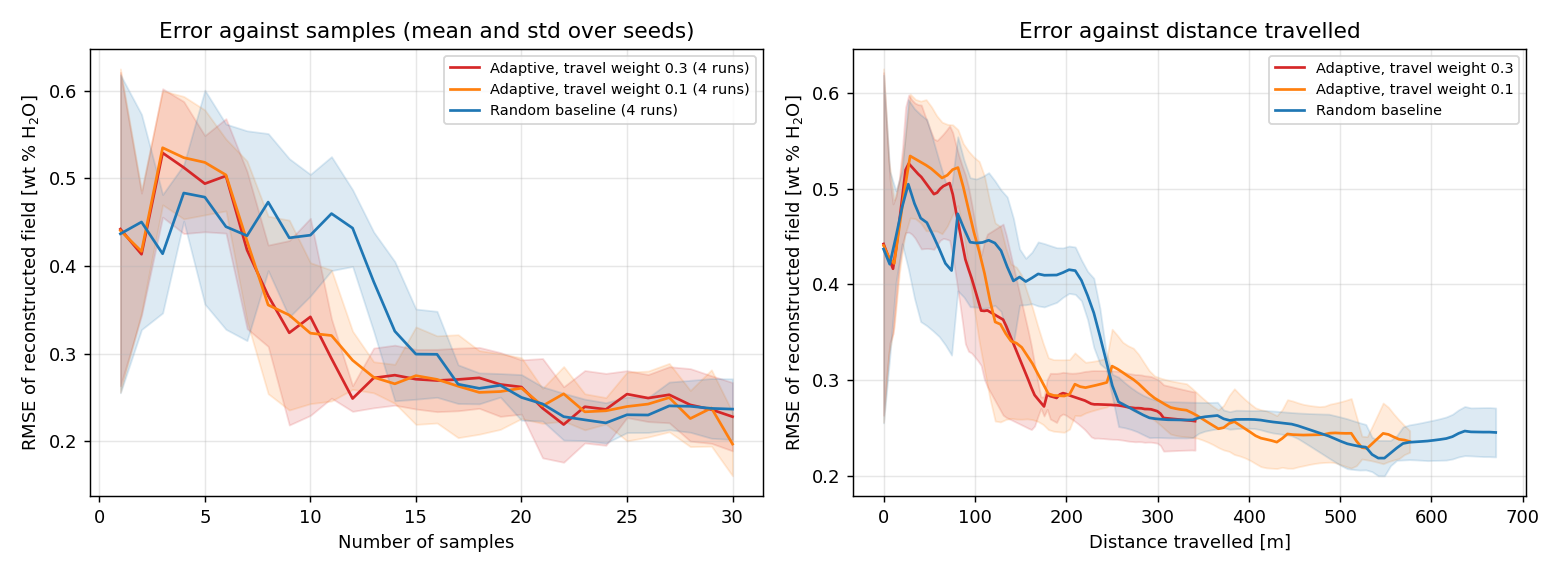
\includegraphics[width=0.85\linewidth]{advanced6_gazebo_multiseed.png}
  \caption{Gazebo runs: error against samples and against distance travelled.}
\end{figure}


\paragraph{How to read the results.}
\begin{itemize}[nosep]
  \item \textbf{Adaptive drives less.} With travel weight 0.3, every adaptive run drove less than every random run
        (341 to 555\,m against 670 to 818\,m). On average that is 477\,m against 735\,m, about 35\% less distance, and
        about 35\% less time (10.5 against 16.1 minutes).
  \item \textbf{Final accuracy is similar.} After 30 readings the average error is 0.228 for adaptive (weight 0.3)
        and 0.237 for random. Seed to seed, the error varies by about 0.04, which is larger than the difference between
        the two strategies, so these results cannot show that one is more accurate than the other.
  \item \textbf{Early accuracy is indicative only.} After 10 readings adaptive averages 0.34 and random 0.44, but one adaptive
        run (seed 3) was as bad as the worst random run at that point (0.54 for both). With four seeds this is not reliable.
  \item \textbf{Reaching a given error takes the same driving.} The average distance at which the error first dropped to
        0.30 was 168\,m for adaptive and 172\,m for random. The saving from adaptive sampling appears after that point: it keeps
        improving with shorter trips, while random sampling keeps crossing the cave.
  \item \textbf{A smaller travel weight did not help.} With weight 0.1 the final error was slightly lower (0.197) but within
        the spread, and the robot drove about 30\% farther (625 against 477\,m). Weight 0.3 is the better choice.
\end{itemize}
In summary, in these runs adaptive sampling gives a survey of similar quality using about two-thirds of the driving
and time. It did not give a more accurate one. Four seeds is a small sample, so a smaller difference could still be hiding
in these numbers.

\todo{Karan: optional: add an RViz screenshot showing the GP mean, uncertainty and true-field overlays, which the screenshot in Figure~\ref{fig:rviz} predates. The sample markers are visible there.}

\subsection{Discussion and limits}
\begin{itemize}[nosep]
  \item In the offline study, adaptive is worse than random after 5 samples, because the travel penalty keeps
        it near the start while the GP extrapolates over unseen cave. It is ahead from about 10 samples
        (clearest at 20: 0.293 against 0.366) and uses about half the distance. By 30 and 40 samples the two
        have the same error (0.250 against 0.250, and 0.215 against 0.217). The reliable advantage is
        therefore less driving, not a lower final error. The Gazebo results below point the same way.
  \item The offline study ignores driving time and navigation failures. The Gazebo runs include them.
  \item Measurement noise (0.23 to 0.36\,wt\% inside the block) is large against the field's range (2.3 to 5.0\,wt\%), which
        puts a floor on the achievable error of about 0.2.
  \item The online error is computed over the cave explored so far, so its region grows during a run.
  \item Possible improvements: choose the travel weight from the remaining sample budget; use the map to
        sample at ridge points rather than a lattice; and a kernel that is not isotropic.
\end{itemize}

% =====================================================================
\section{Results}
\label{sec:results}

\begin{notebox}[STUDENT ACTION REQUIRED --- all]
Describe what was achieved overall, with pictures, graphs or plots as evidence of a working system. Include the
video link below. The report lead will assemble this once all parts are on the shared repository and have
been run together.
\end{notebox}

\paragraph{Summary of what has been shown, by part.}
\begin{itemize}[nosep]
  \item \textbf{Advanced 2:} widest area and passages found and displayed on the real SLAM map
        (Figure~\ref{fig:a2slam}).
  \item \textbf{Advanced 6:} 12 runs of 30 readings completed in Gazebo with real navigation (4 seeds, 3 settings); offline
        comparison over 10 runs (Section~\ref{sec:advanced6}).
  
  \item \textbf{Perception:} \todo{Andrew: add Perception results and a figure.} The stop-sign classifier found 28 of 32 clear views
        of the five signs, with no false boxes on the poster walls (Section~\ref{sec:perception}).
  \item \textbf{Planning:} Planning 1--3 were tested in ROS~2 Humble with Gazebo, RViz and Nav2. The rover generated
        frontier goals, switched to close-range inspection of artefacts and resumed exploration. In two runs of the finished node,
        all five stop signs were inspected with no stuck events (Section~\ref{sec:integration}). Complete cave coverage and recovery
        from every failure were not verified.
\end{itemize}

\paragraph{Video.}
\todo{Link to the video(s). Upload to YouTube, OneDrive or Google Drive and check that the marker can open it. If
several short videos are submitted, say so here and list them. About five minutes in total.}

% =====================================================================
\section{Reflection on Teamwork}

\begin{notebox}[Write this from your own experience]
The points below are taken from the repository history. Each member should add a specific and accurate account of their own experience.
\end{notebox}

\begin{itemize}[nosep]
  \item \textbf{Plan.} The team agreed on a split by task block (Perception, Planning, Advanced), with dated checkpoints and a list of what
        each member owes the others. The repository shows the first contributions from Perception on 11~October and from Planning on 12~October, after the
        first planned checkpoints (6 to 10~October).
  \item \textbf{Shared repository.} Two versions of the shared exploration node were developed in parallel, one on \texttt{main} and one on the
        \texttt{planning} branch. They had to be reconciled by hand. The merged version keeps the planning behaviour and replaces the version that was on \texttt{main}. The Perception edit on \texttt{main} is not part of the merged node. The Advanced work is in separate
        nodes, so it does not edit the shared node.
  \item \textbf{Dependencies.} The Planning node needs the position of each artefact from Perception~3, which is not yet on the repository.
        The integrated node therefore measures the position of each stop sign with the depth camera (Section~\ref{sec:integration}).
  \item \textbf{Integration.} The autonomy launch runs exploration, inspection and the stop-sign detector together. Perception~1--3 and the
        other artefact detectors are not part of that run.
  
\item \textbf{What each member learned.}

\textbf{Christina Li:} I learned that developing a planning algorithm is only part of building an autonomous robotic system. Testing Planning 1--3 in Gazebo showed me how important navigation feedback, error handling and coordination with the perception module are. I also learned to verify the robot's behaviour through simulation logs and RViz rather than relying only on the code.

\textbf{Andrew Than:} \todo{Andrew: add your own reflection.}

\textbf{Karan Sharma:} \todo{Karan: add your own reflection.}

\end{itemize}


% =====================================================================
% The bibliography below prints its own "References" heading
\addcontentsline{toc}{section}{References}
\begin{thebibliography}{9}
\bibitem{pds} W.~V. Boynton. \emph{2001 Mars Odyssey Gamma Ray Spectrometer Element Concentration Data}. NASA Planetary Data System,
  data set ODY-M-GRS-5-ELEMENTS-V1.0, 2007 (product H2O\_SR\_5X5). This is the citation given in the data set's own catalogue.
  \url{https://pds-geosciences.wustl.edu/ody/ody-m-grs-5-elements-v1/odgm_xxxx/}. Downloaded 5 October 2026.
\bibitem{pds_catalog} NASA Planetary Data System. Catalogue files of the same data set (\texttt{inst.cat}, \texttt{mission.cat}): instrument description, mapping orbit
  of 400\,km, and sensing depth of the upper few tens of centimetres. Read 12 October 2026.
\bibitem{boynton2007} W.~V. Boynton et al. ``Concentration of H, Si, Cl, K, Fe, and Th in the low- and mid-latitude regions of Mars.''
  \emph{Journal of Geophysical Research: Planets}, 112(E12), 2007. doi:10.1029/2007JE002887.
\bibitem{boynton2004} W.~V. Boynton et al. ``The Mars Odyssey Gamma-Ray Spectrometer instrument suite.''
  \emph{Space Science Reviews}, 110(1--2), 37--83, 2004. doi:10.1023/B:SPAC.0000021007.76126.15.
\bibitem{feldman2004} W.~C. Feldman et al. ``Global distribution of near-surface hydrogen on Mars.''
  \emph{Journal of Geophysical Research: Planets}, 109(E9), 2004. doi:10.1029/2003JE002160.
\bibitem{mitrofanov2012} I.~Mitrofanov et al. ``Dynamic Albedo of Neutrons (DAN) experiment onboard NASA's Mars Science Laboratory.''
  \emph{Space Science Reviews}, 170(1--4), 559--582, 2012. doi:10.1007/s11214-012-9924-y.
\bibitem{wiki_arsia} ``Arsia Mons''. Wikipedia. \url{https://en.wikipedia.org/wiki/Arsia_Mons}. Position 8.35$^{\circ}$S, 239.91$^{\circ}$E.
  Read 12 October 2026.
\end{thebibliography}

\end{document}
